\section{Presentation Logic Layer}
\graphicspath{ {./HW_1/images/} }
%What pages will be present in your project? briefly indicate how your web site will be organized

The website will be divided into the following pages:
\begin{enumerate}
    \item Homepage: contains information on previous constructions made by the ride constructor. Developed via
jsp.
    \item Login page: allows the users login to the web application. Developed via jsp.
    \item Registration page: allows the user to register to the web pages..
    \item Search maintenance page: allows users to search for maintenance events. written in HTML with the
support of javascript.
    \item Insert maintenance page: allows to insert a new maintenance event. Written in HTML.
    \item Insert measurement file page: allows to upload a file containing the measurements. Written in HTML.
    \item Builder page: allows to redirect users toward pages handling specific resources. Written in HTML.
    \item 2 pages each to handle insertion and update of parks, rides and models. Written in HTML.
    \item Administration page: allows to administrate users’ accounts. Written in HTML.
    \item A support page which displays messages upon completion of specific tasks, such as the removal or update
of resources.
\end{enumerate}

\subsection{Home Screen}
\caption{Home Screen of web contain side bar and some detail about web with login and registration button.About button redirect you to about page of web and Contact Us redirect to Contact Us page.}
\\
%For the main pages put a mockup and describe it in detail.

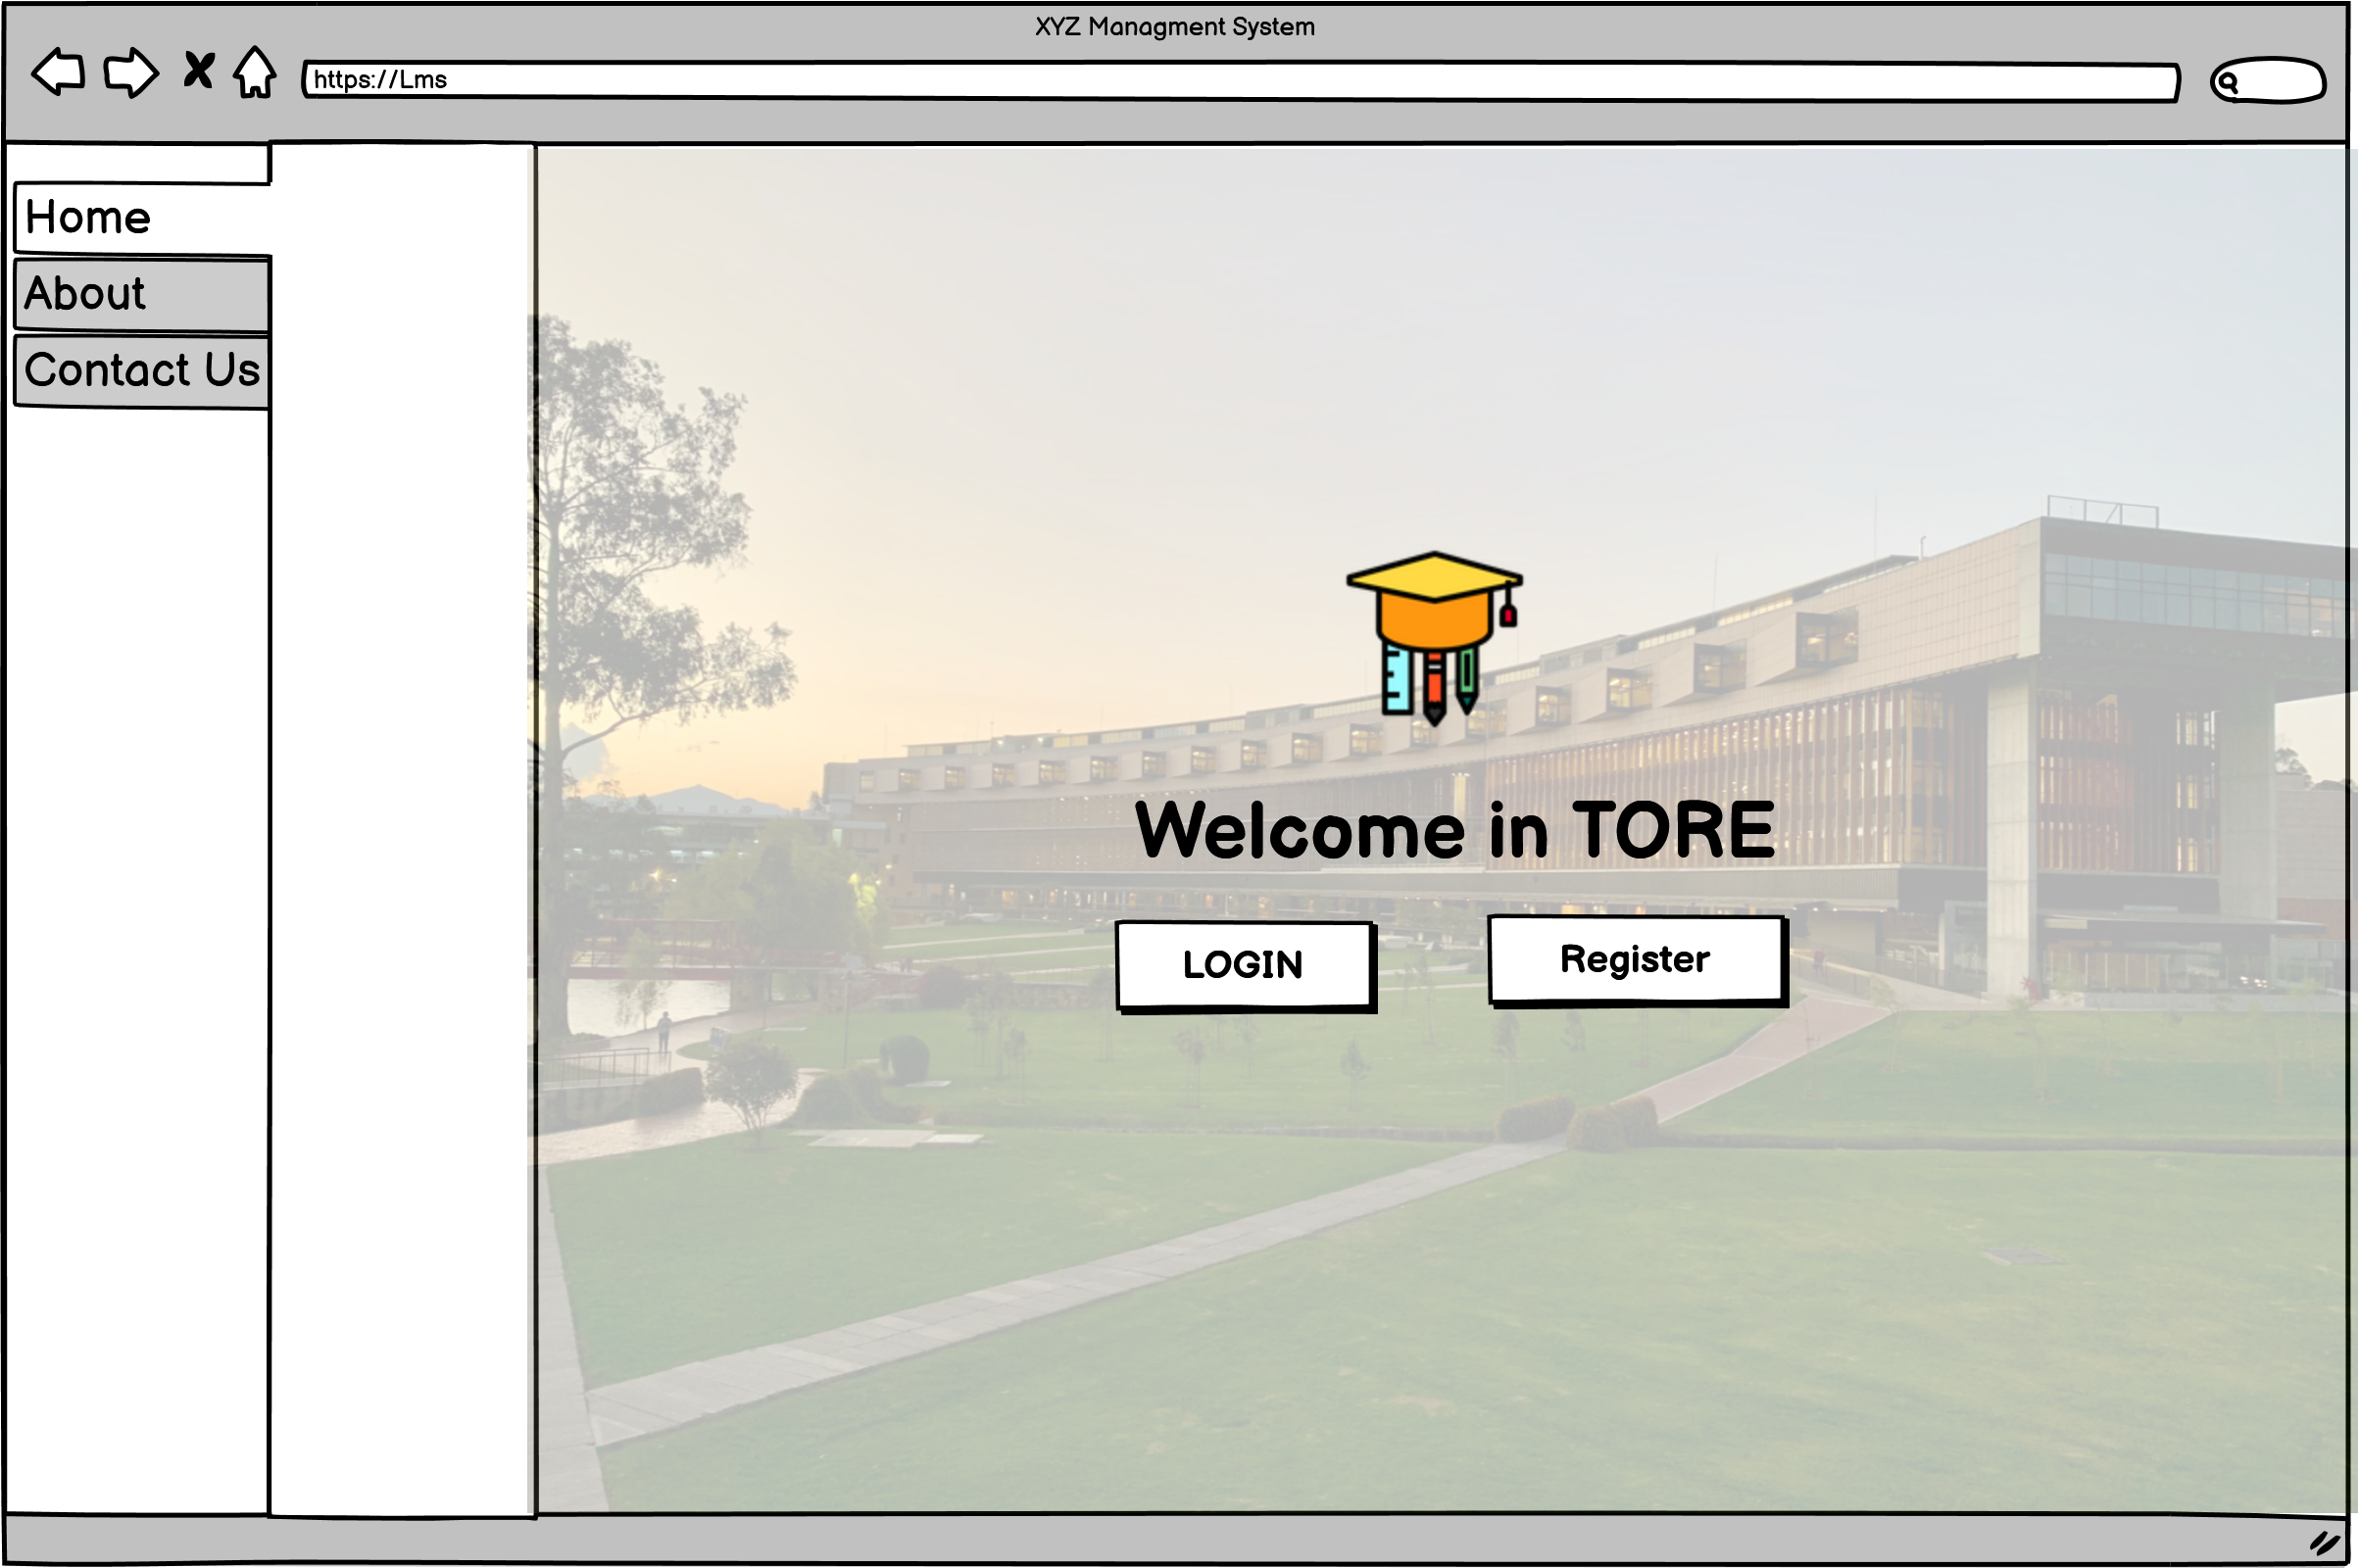
\includegraphics[width=15cm, height=10cm]{HW_1/images/New Wireframe 1.png}


\subsection{Contact Us}
\caption{In Contact Us page user can send message or query direct to institute.}
\\
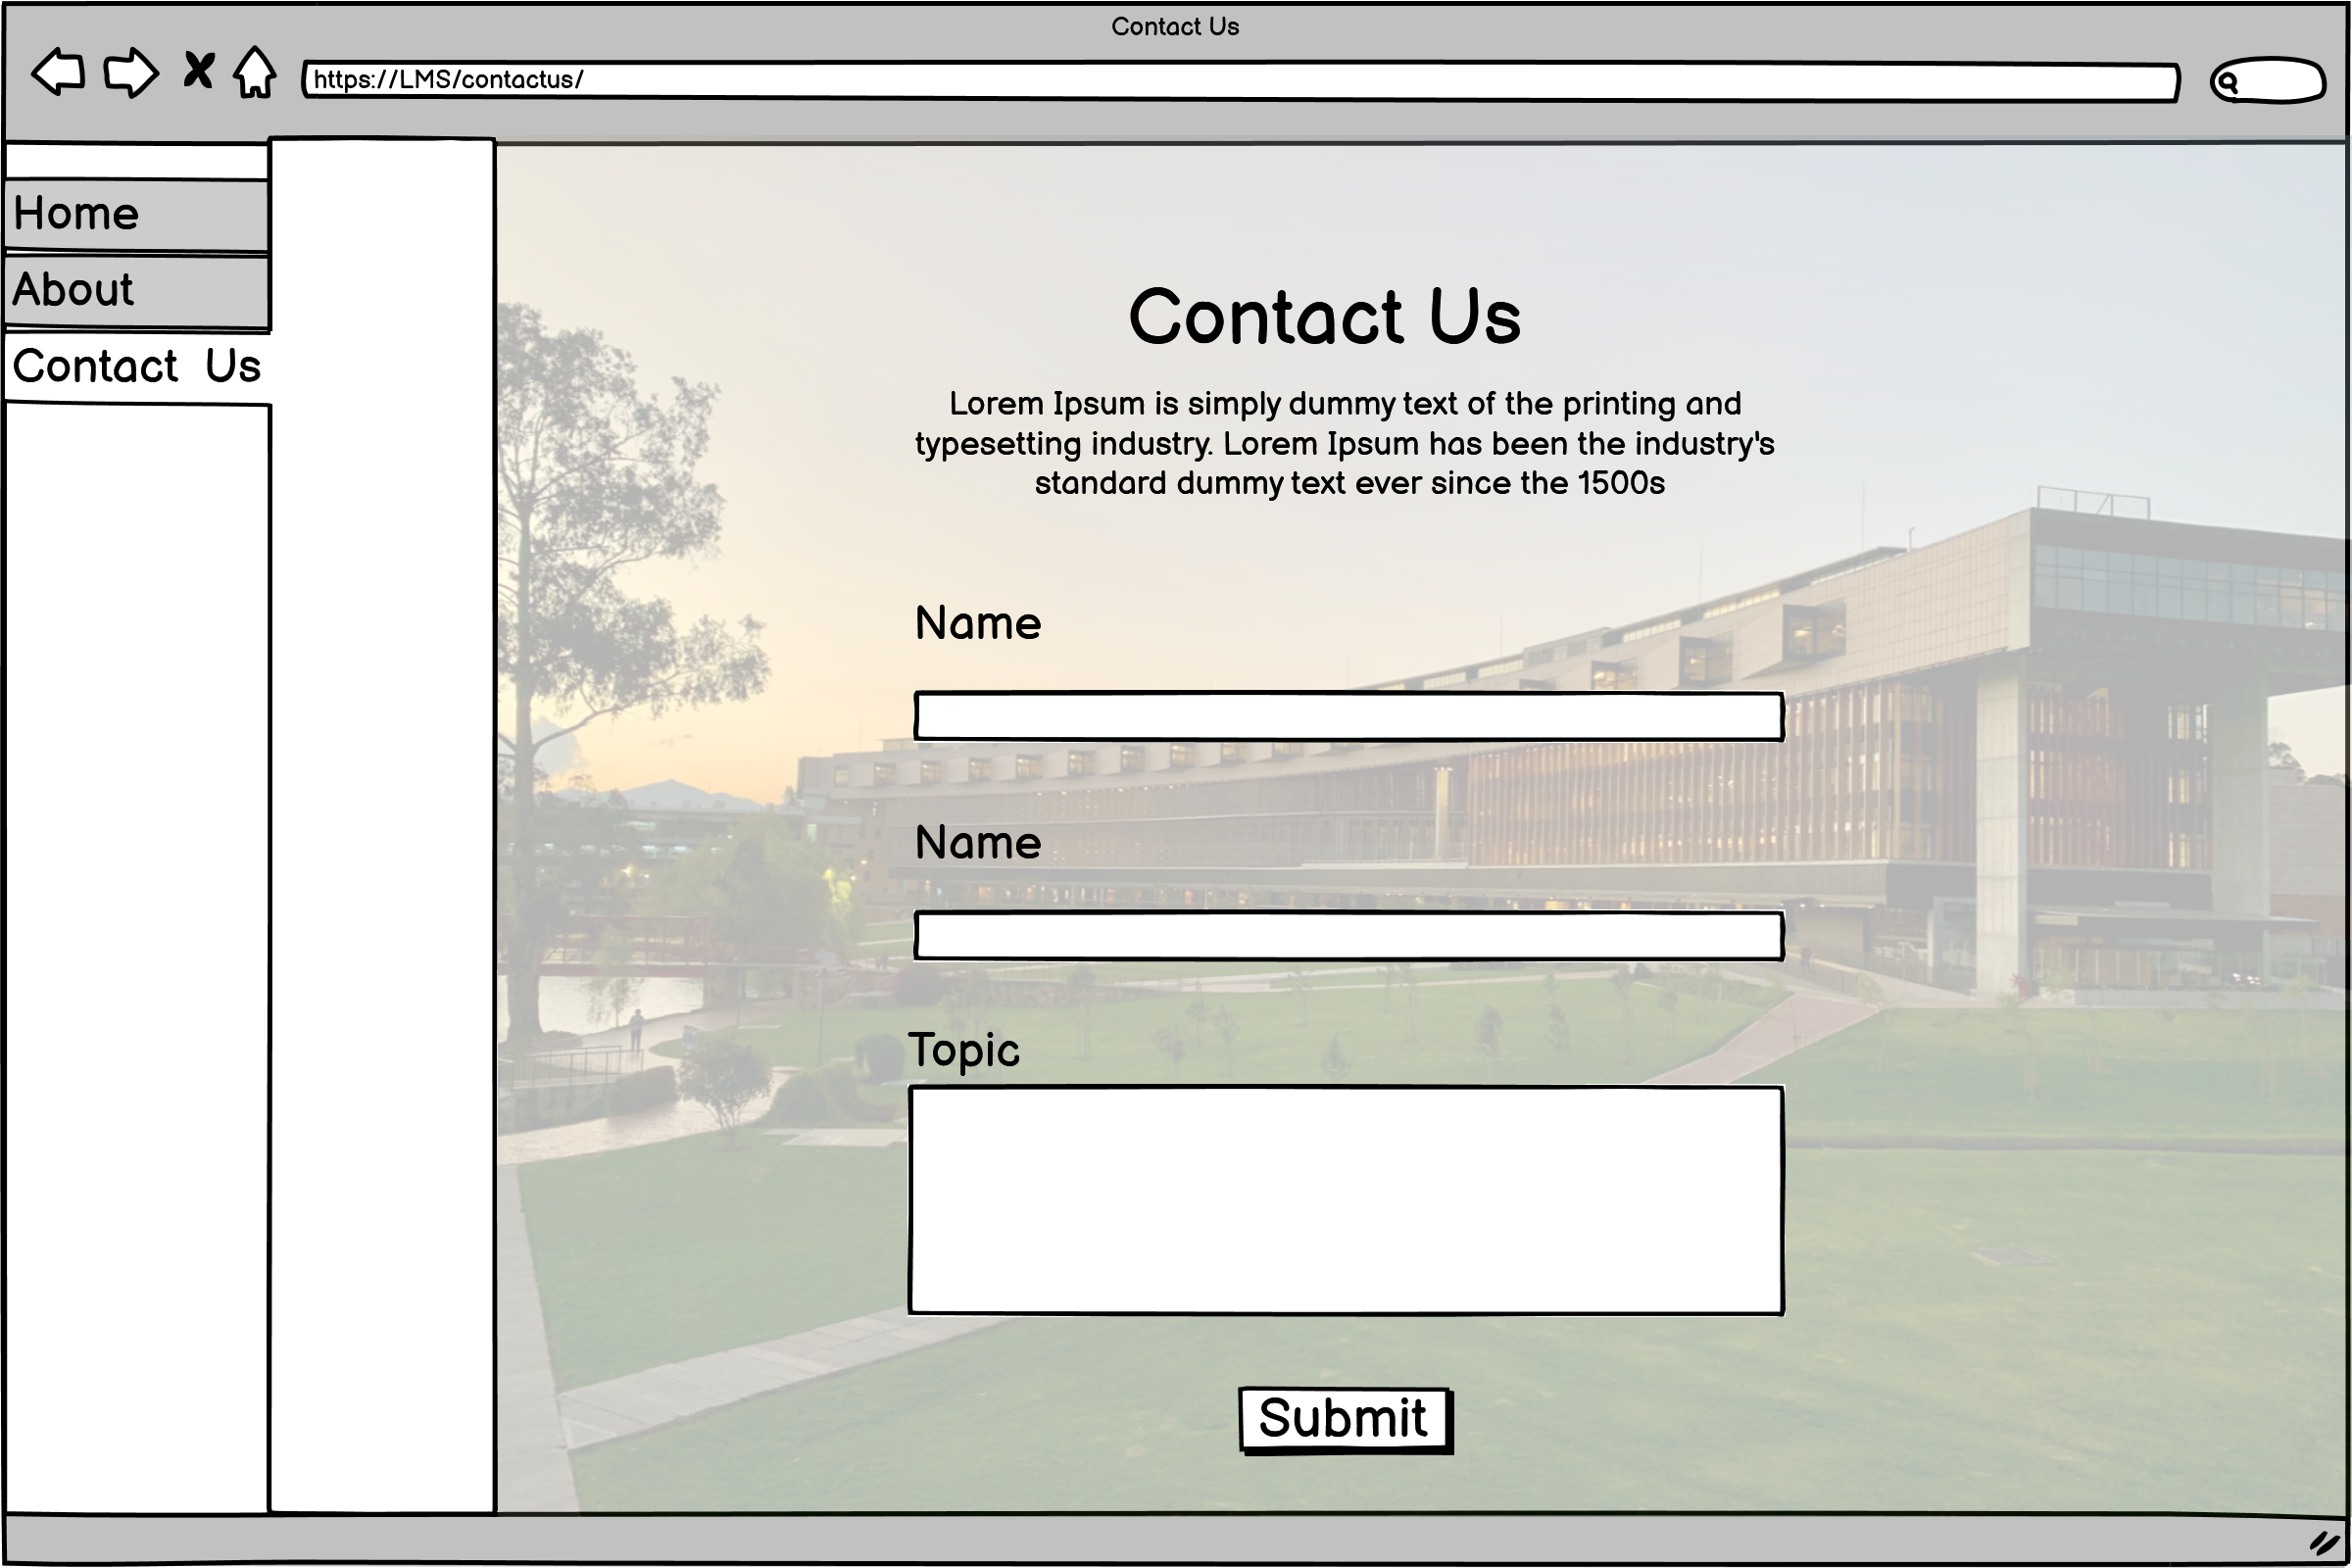
\includegraphics[width=18cm, height=11cm]{HW_1/images/New Wireframe 3.png}

\subsection{About Us}
\caption{About Us page contains the detail of the institute.like Emails, facebook and so on }
\\
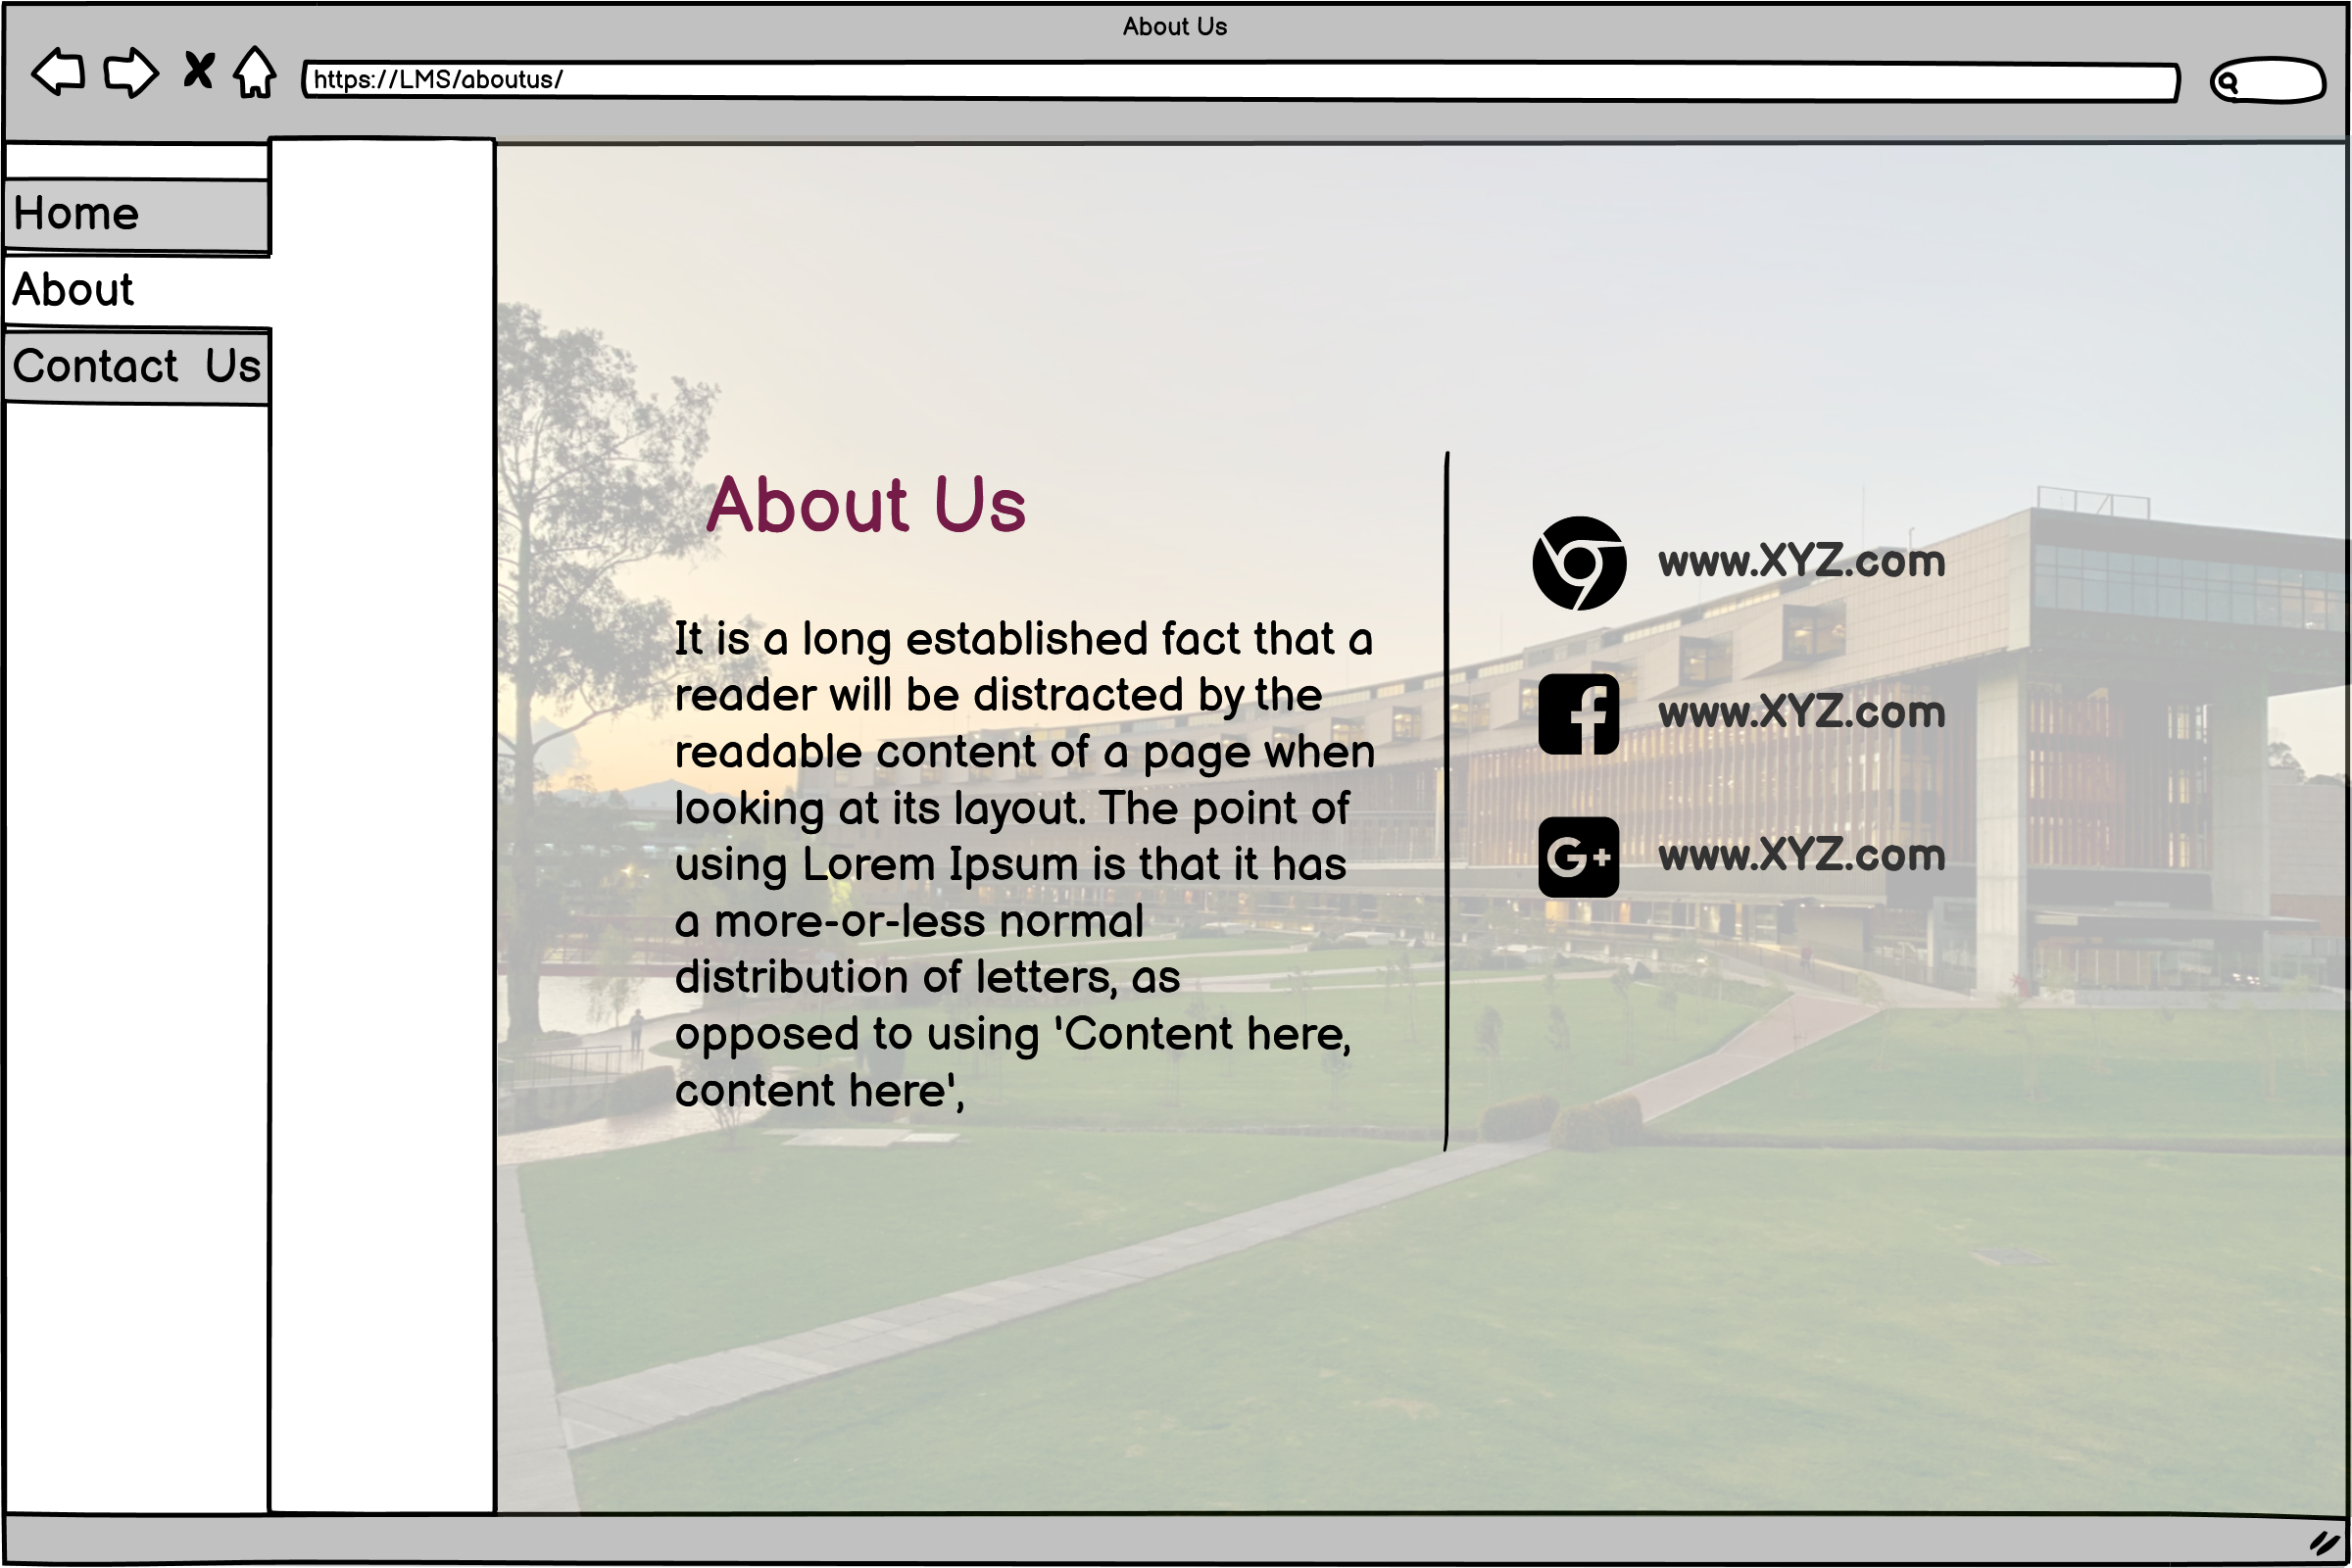
\includegraphics[width=18cm, height=11cm]{HW_1/images/New Wireframe 2.png}


\subsection{Admin Page}

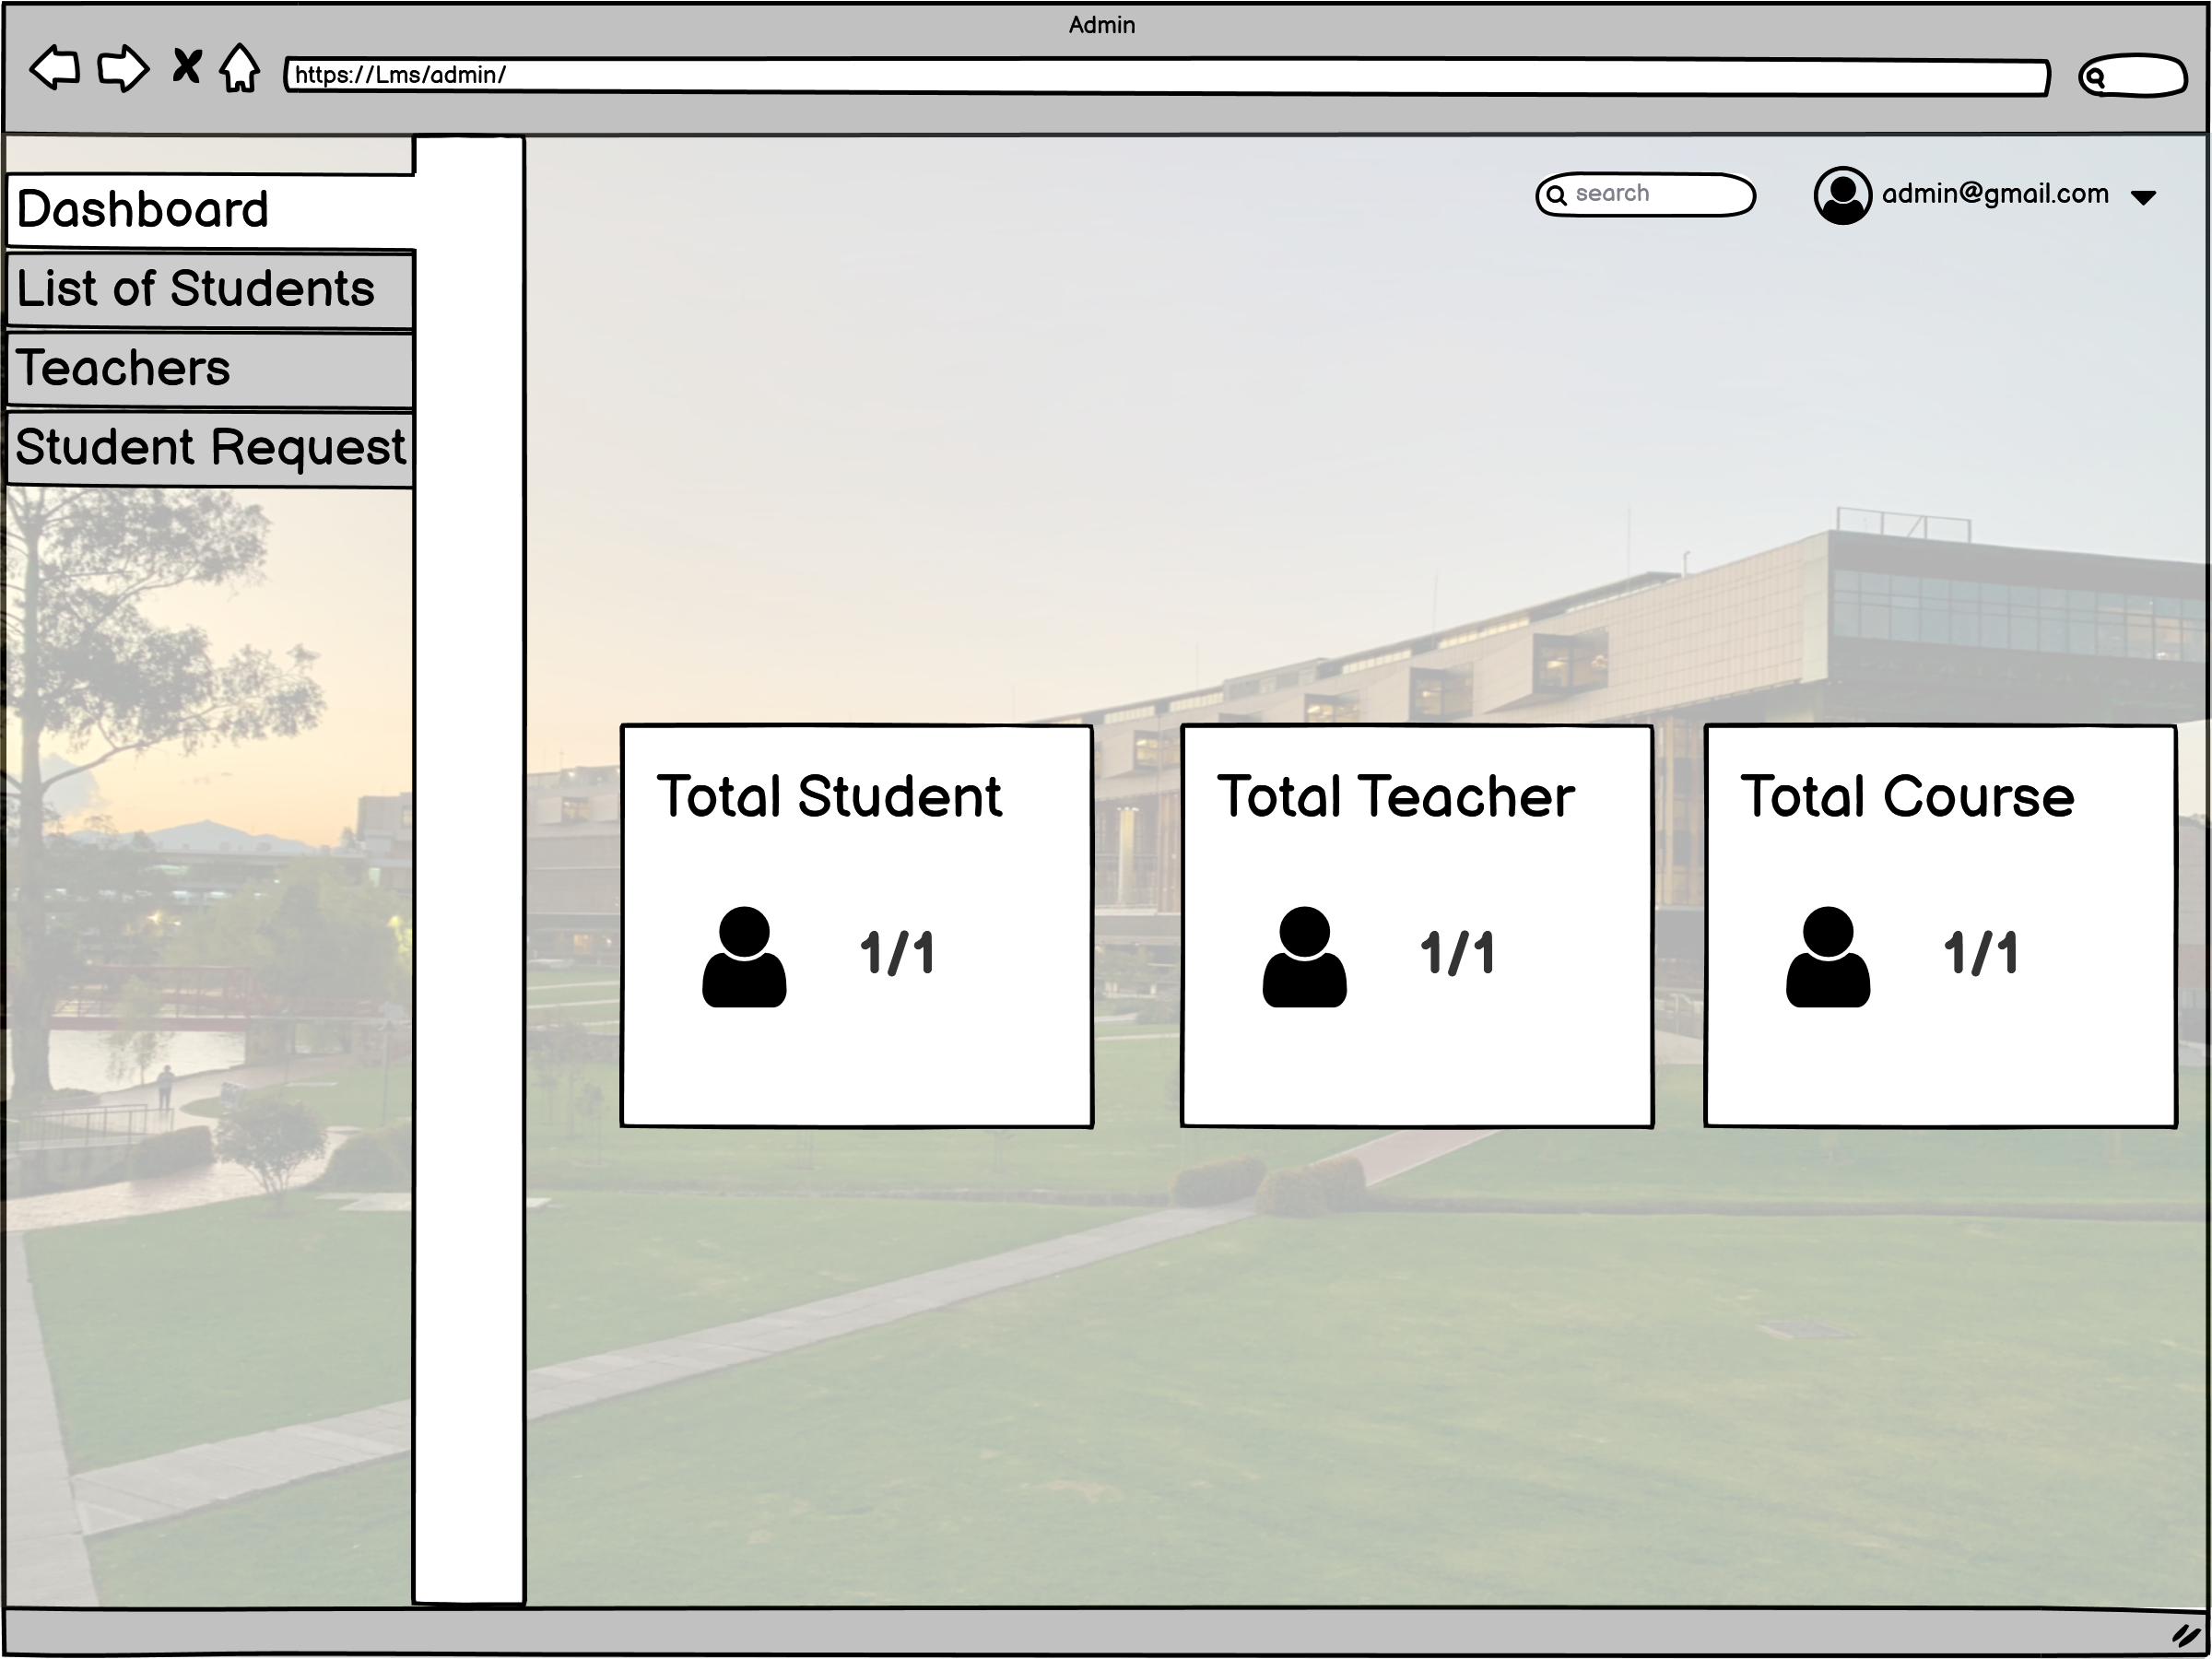
\includegraphics[width=18cm, height=11cm]{HW_1/images/Admin Page.png}

\subsection{List of Students}

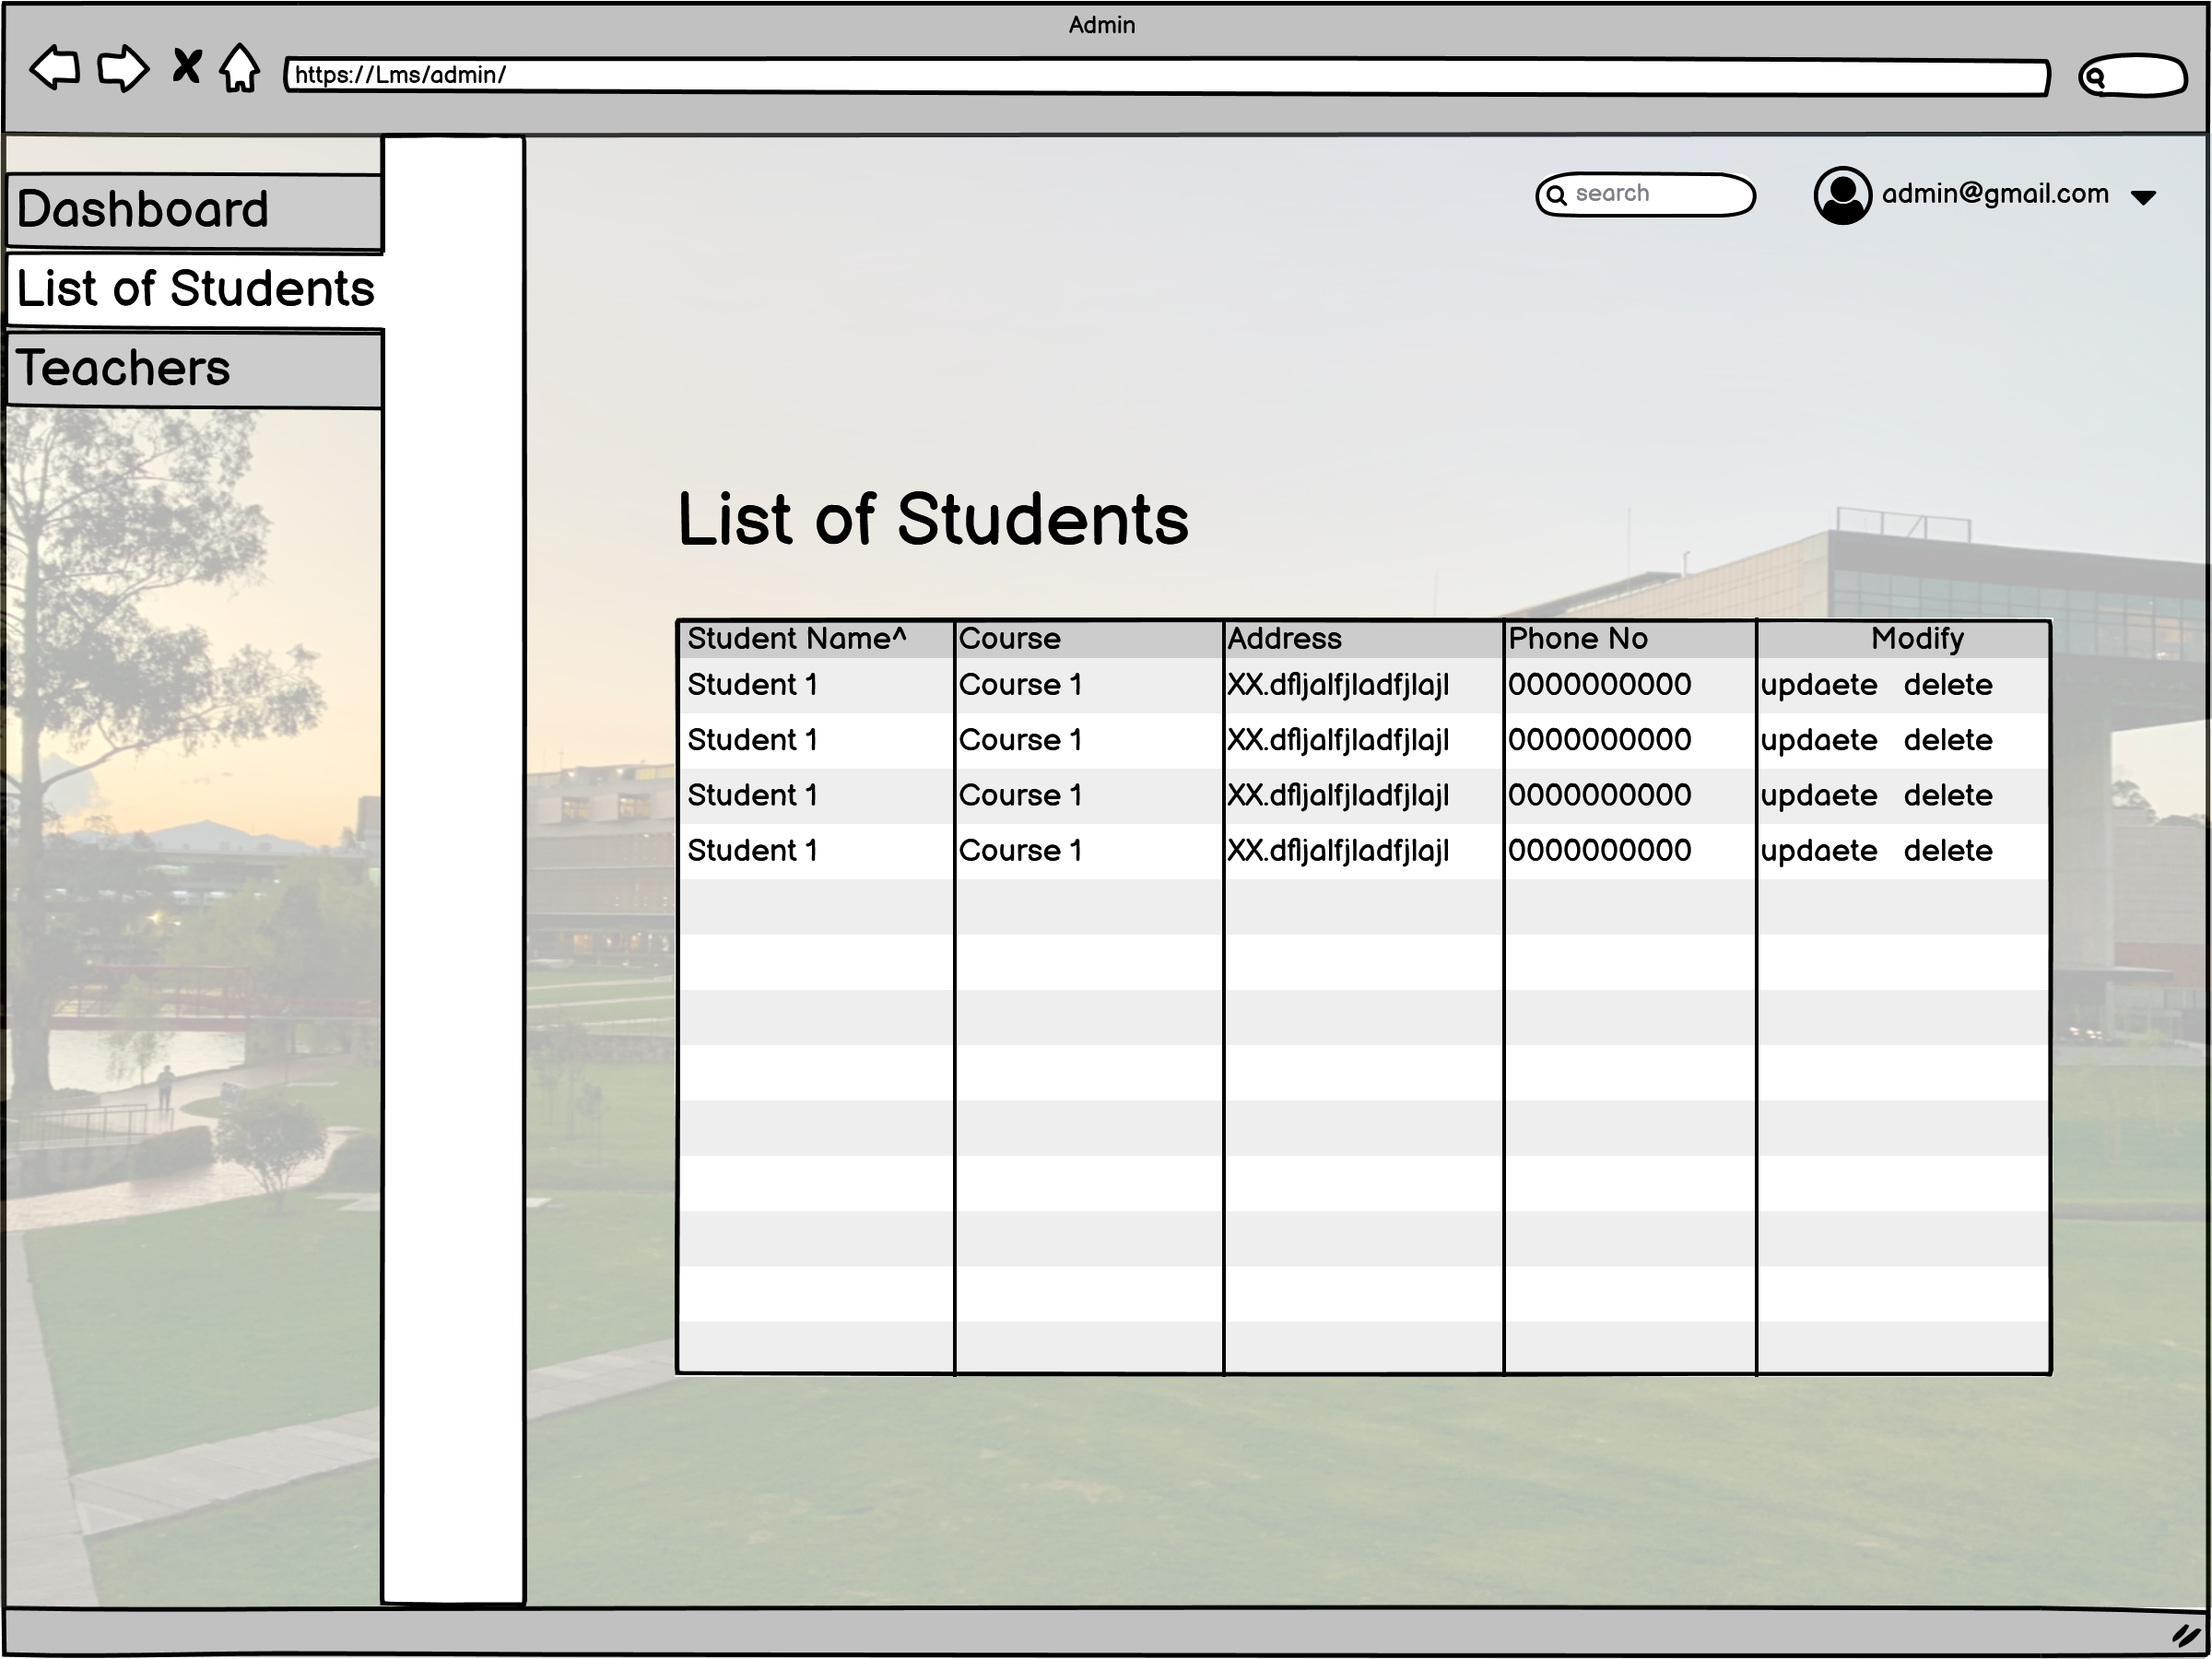
\includegraphics[width=18cm, height=11cm]{HW_1/images/List of Students.png}

\subsection{List of Available Teachers}

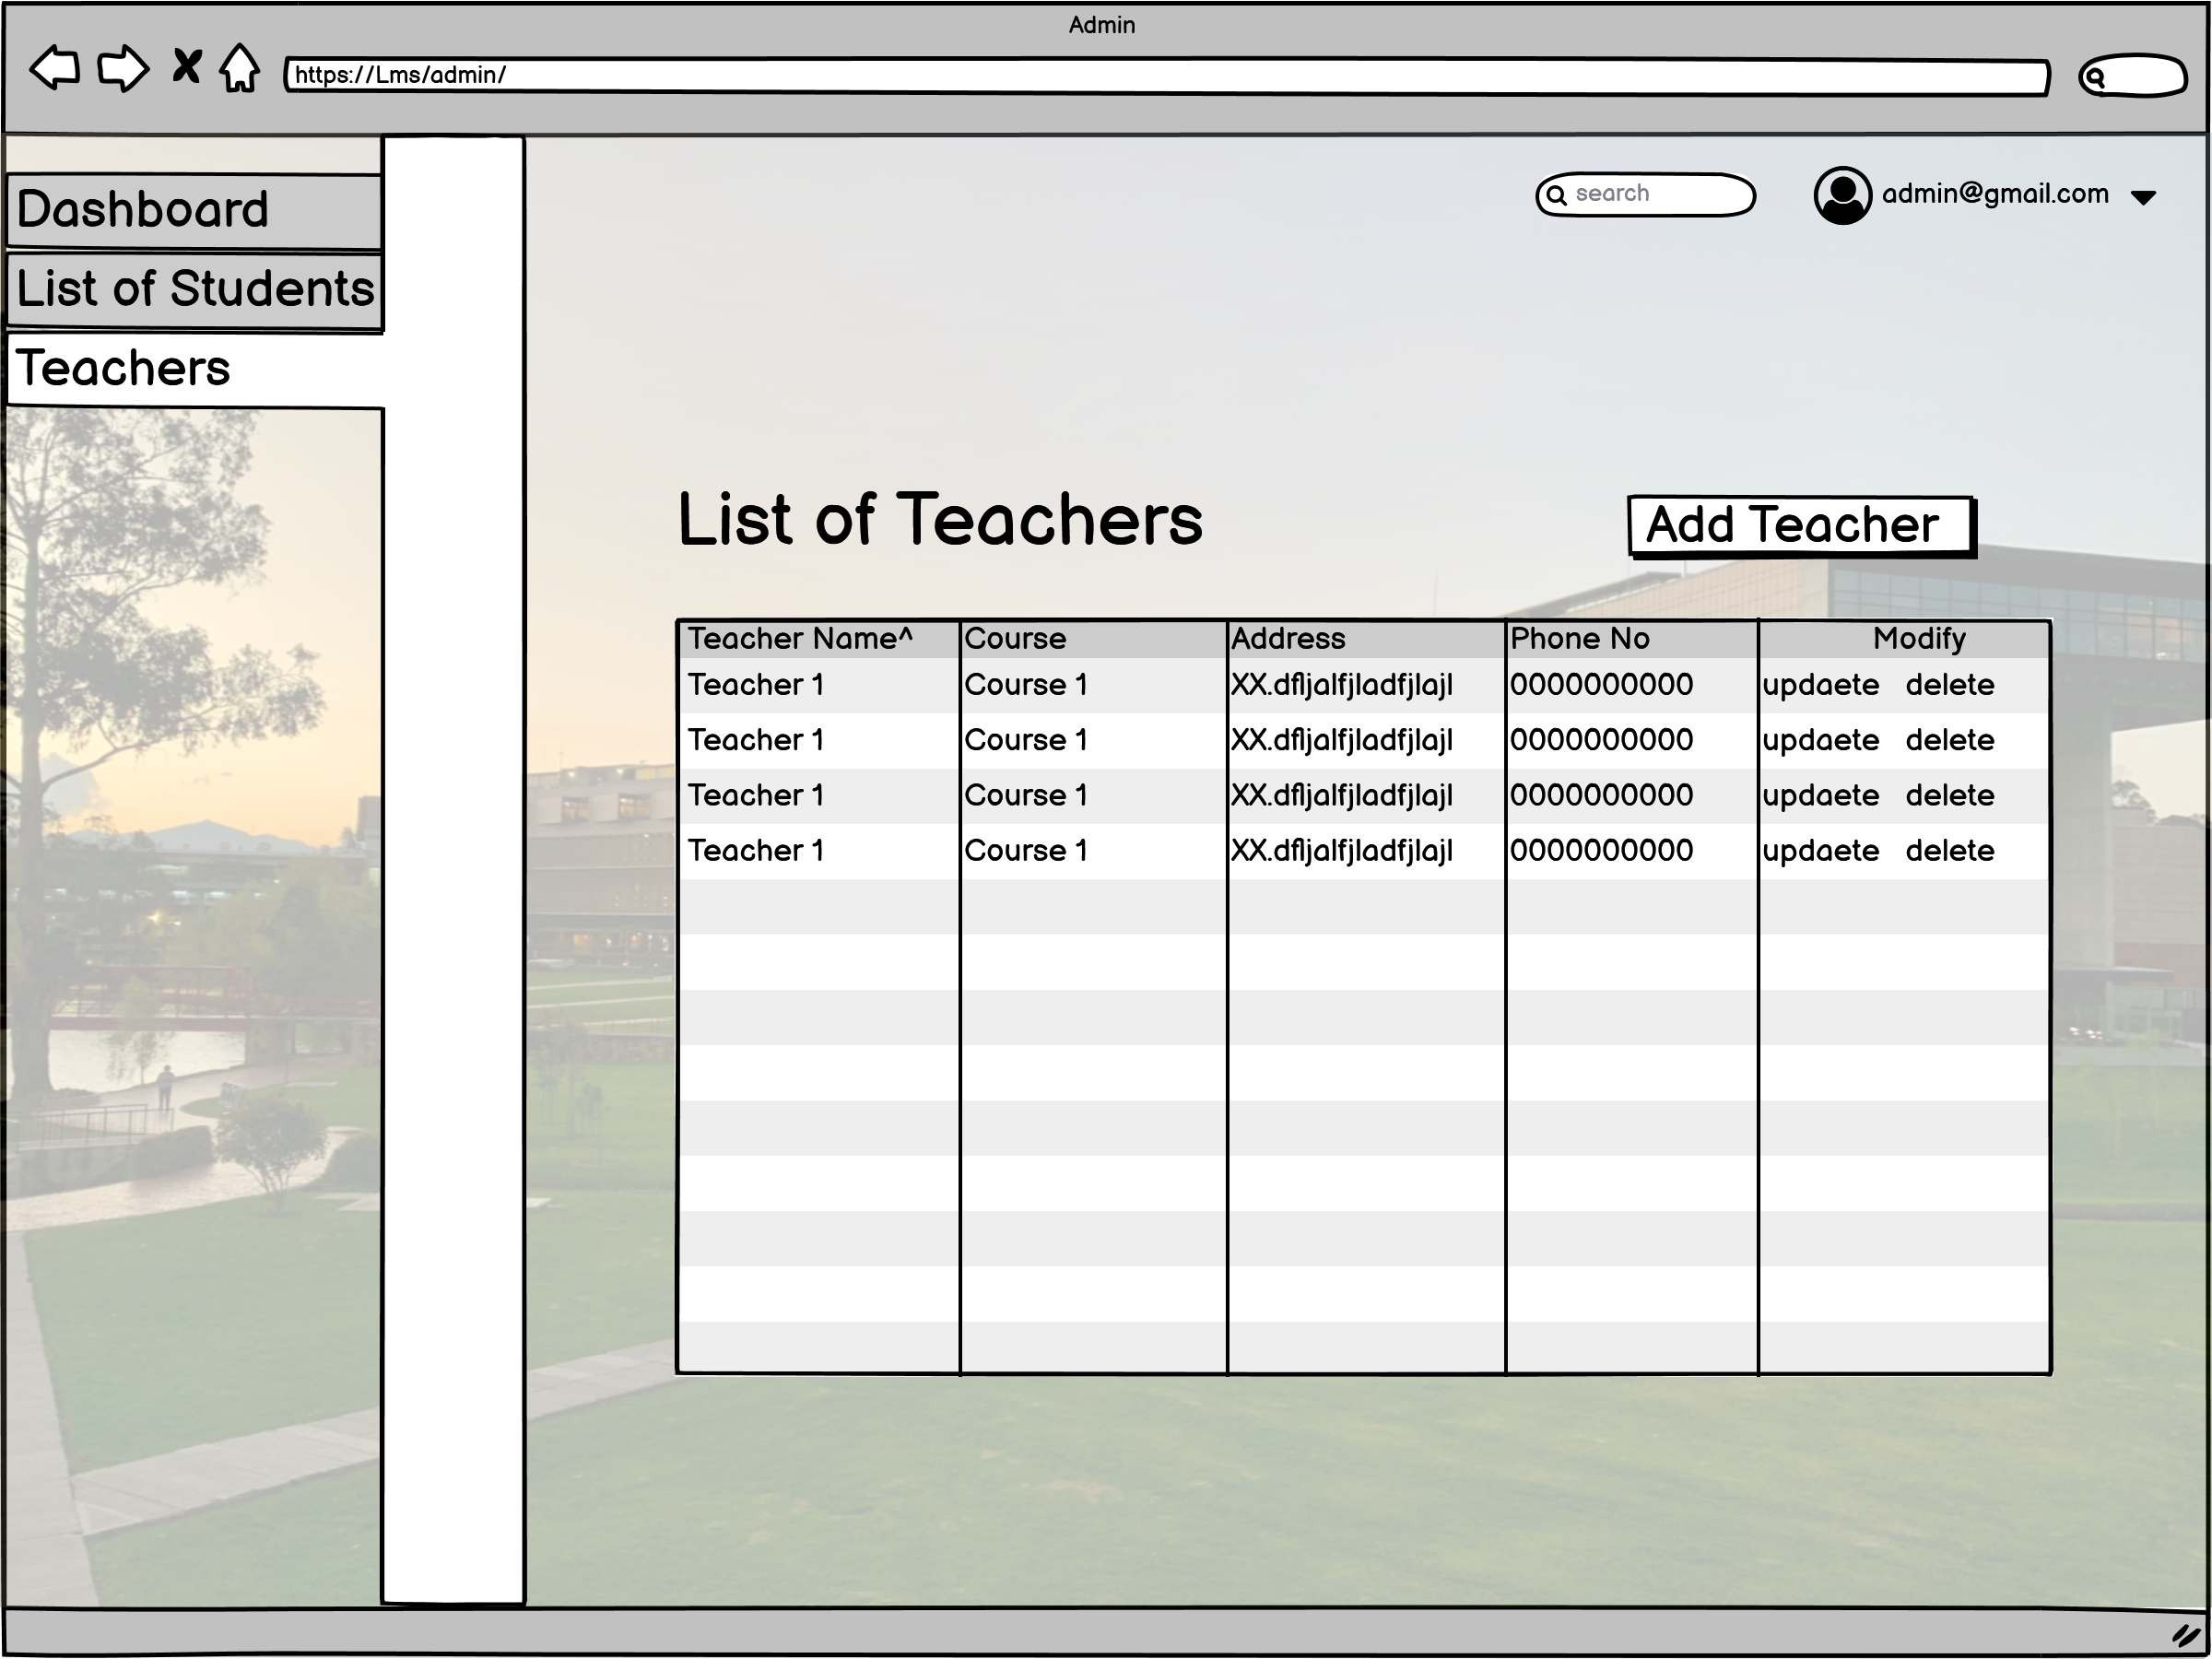
\includegraphics[width=18cm, height=11cm]{HW_1/images/Teachers.png}

\subsection{Teacher Dashboard}

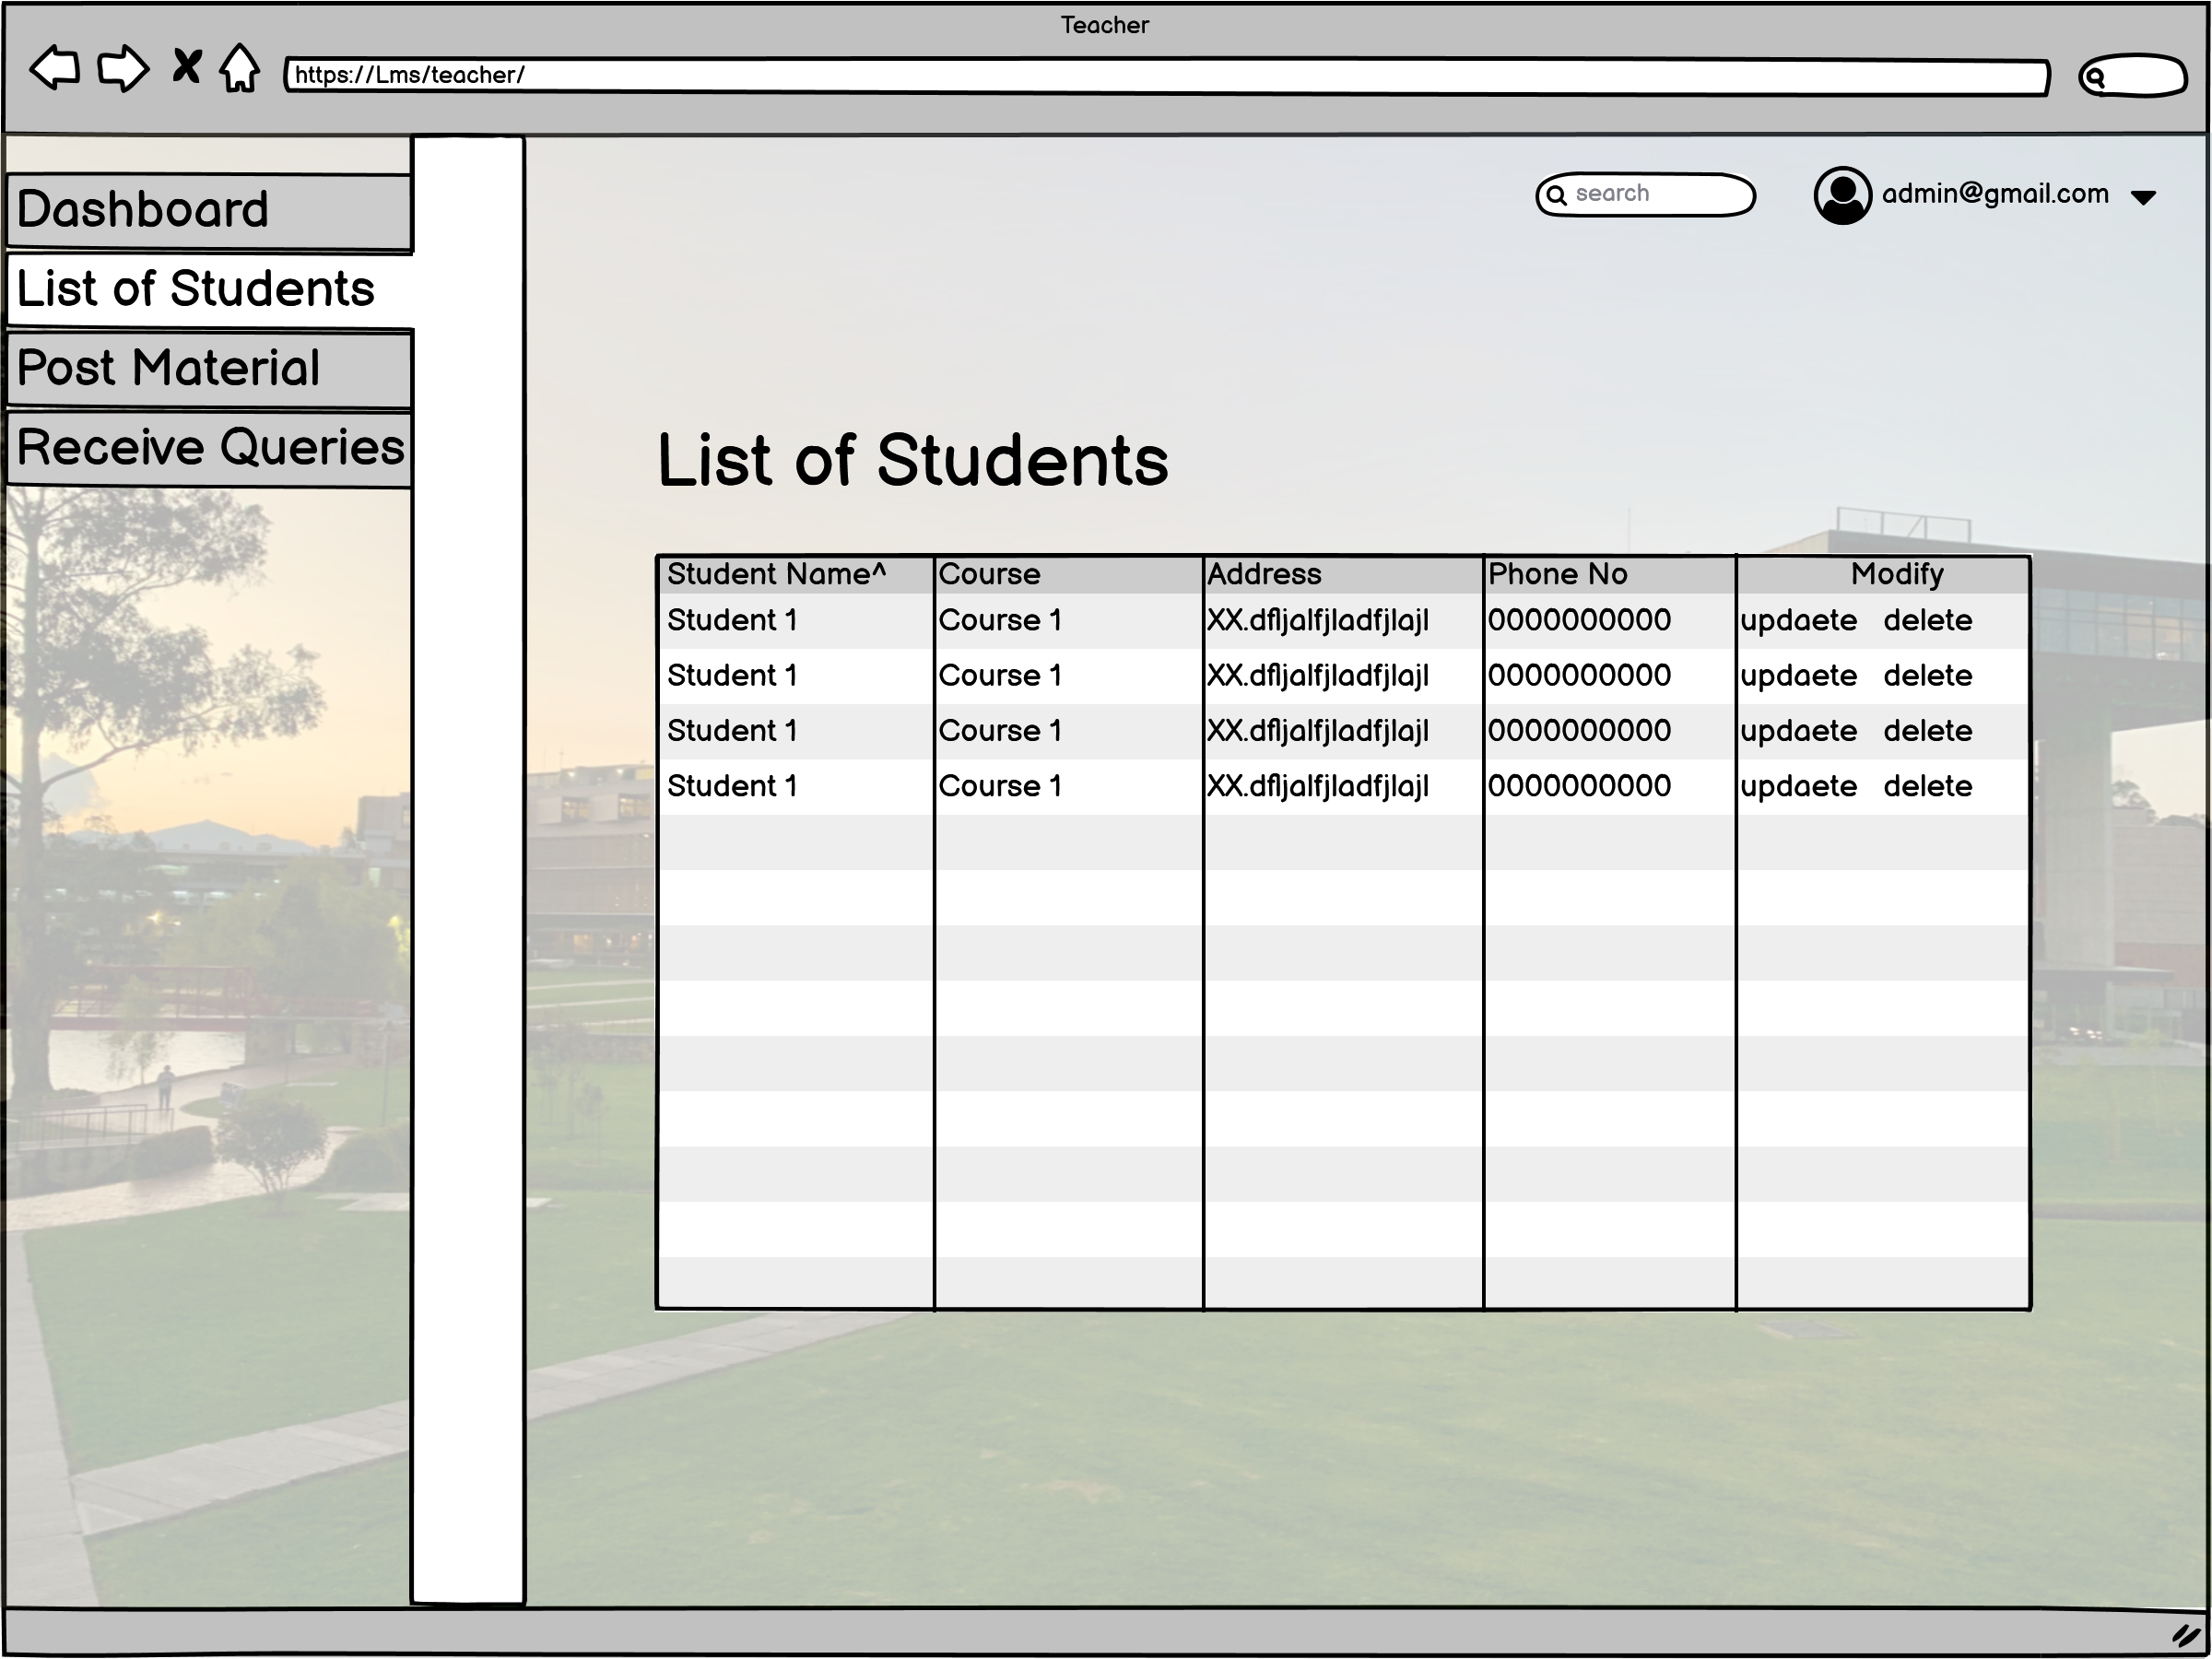
\includegraphics[width=18cm, height=11cm]{HW_1/images/List of Students teacher.png}

\subsection{Available Teachers Page}

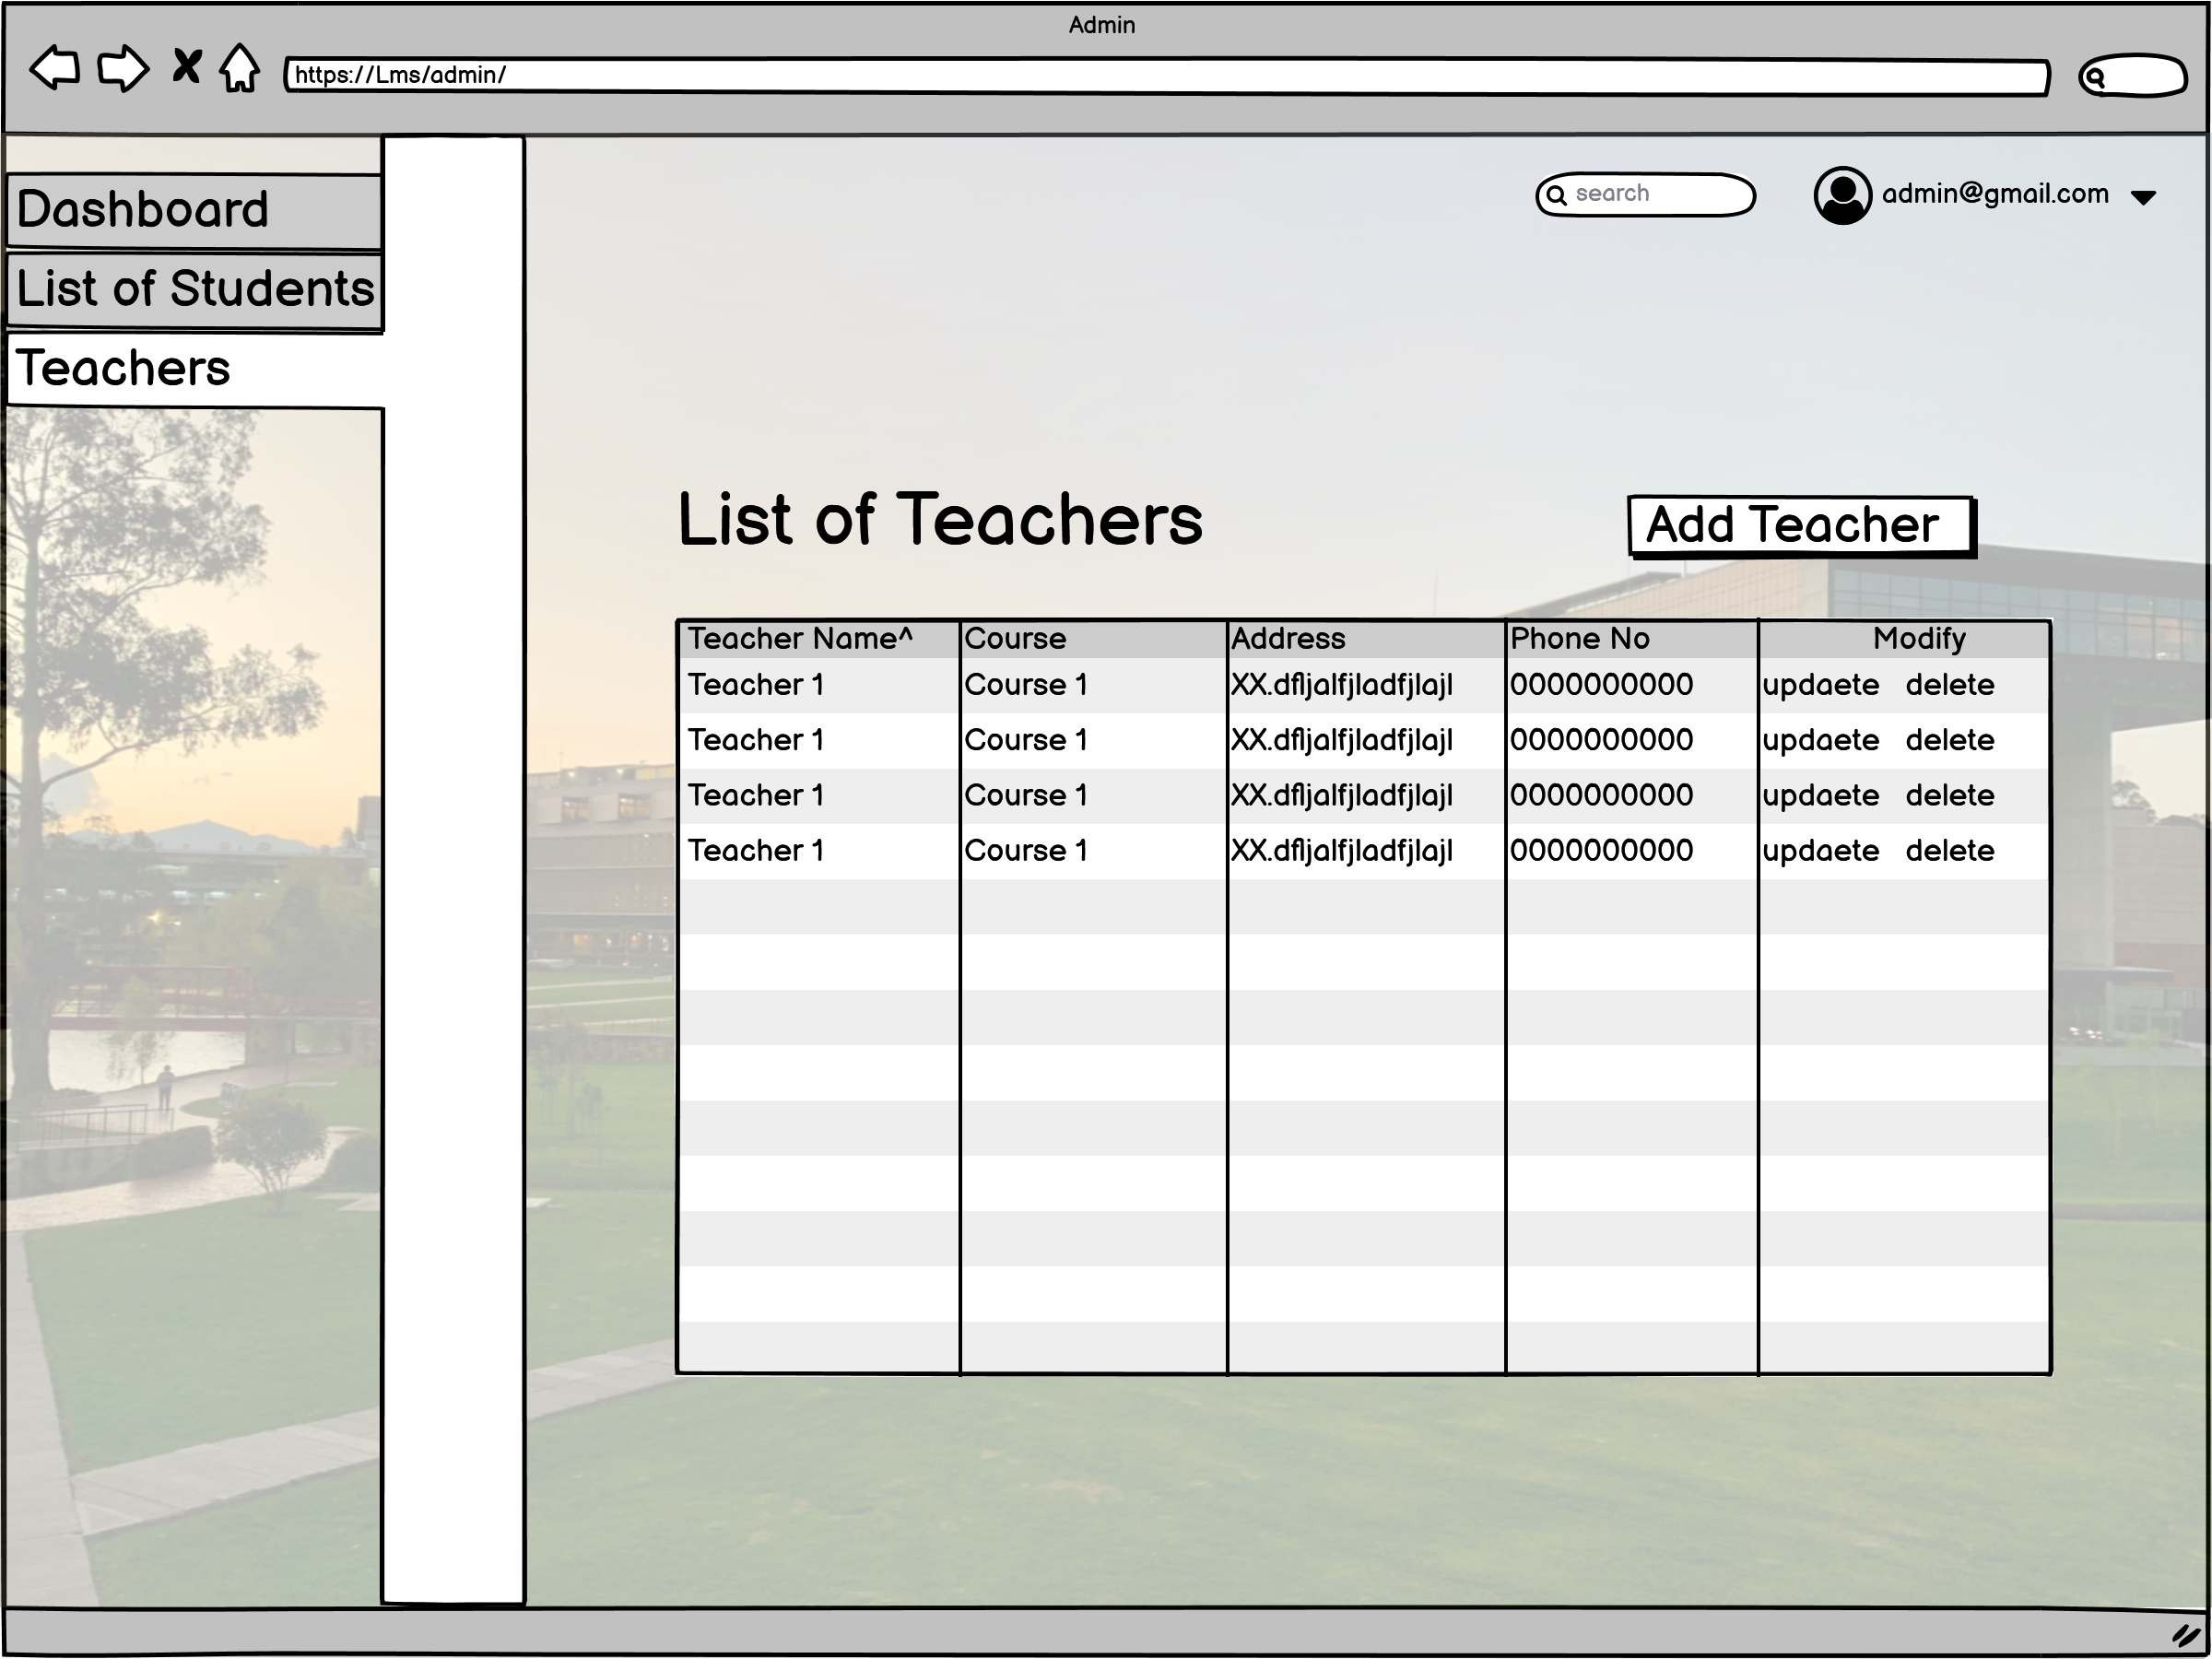
\includegraphics[width=18cm, height=11cm]{HW_1/images/Teachers.png}

\subsection{Home Page}

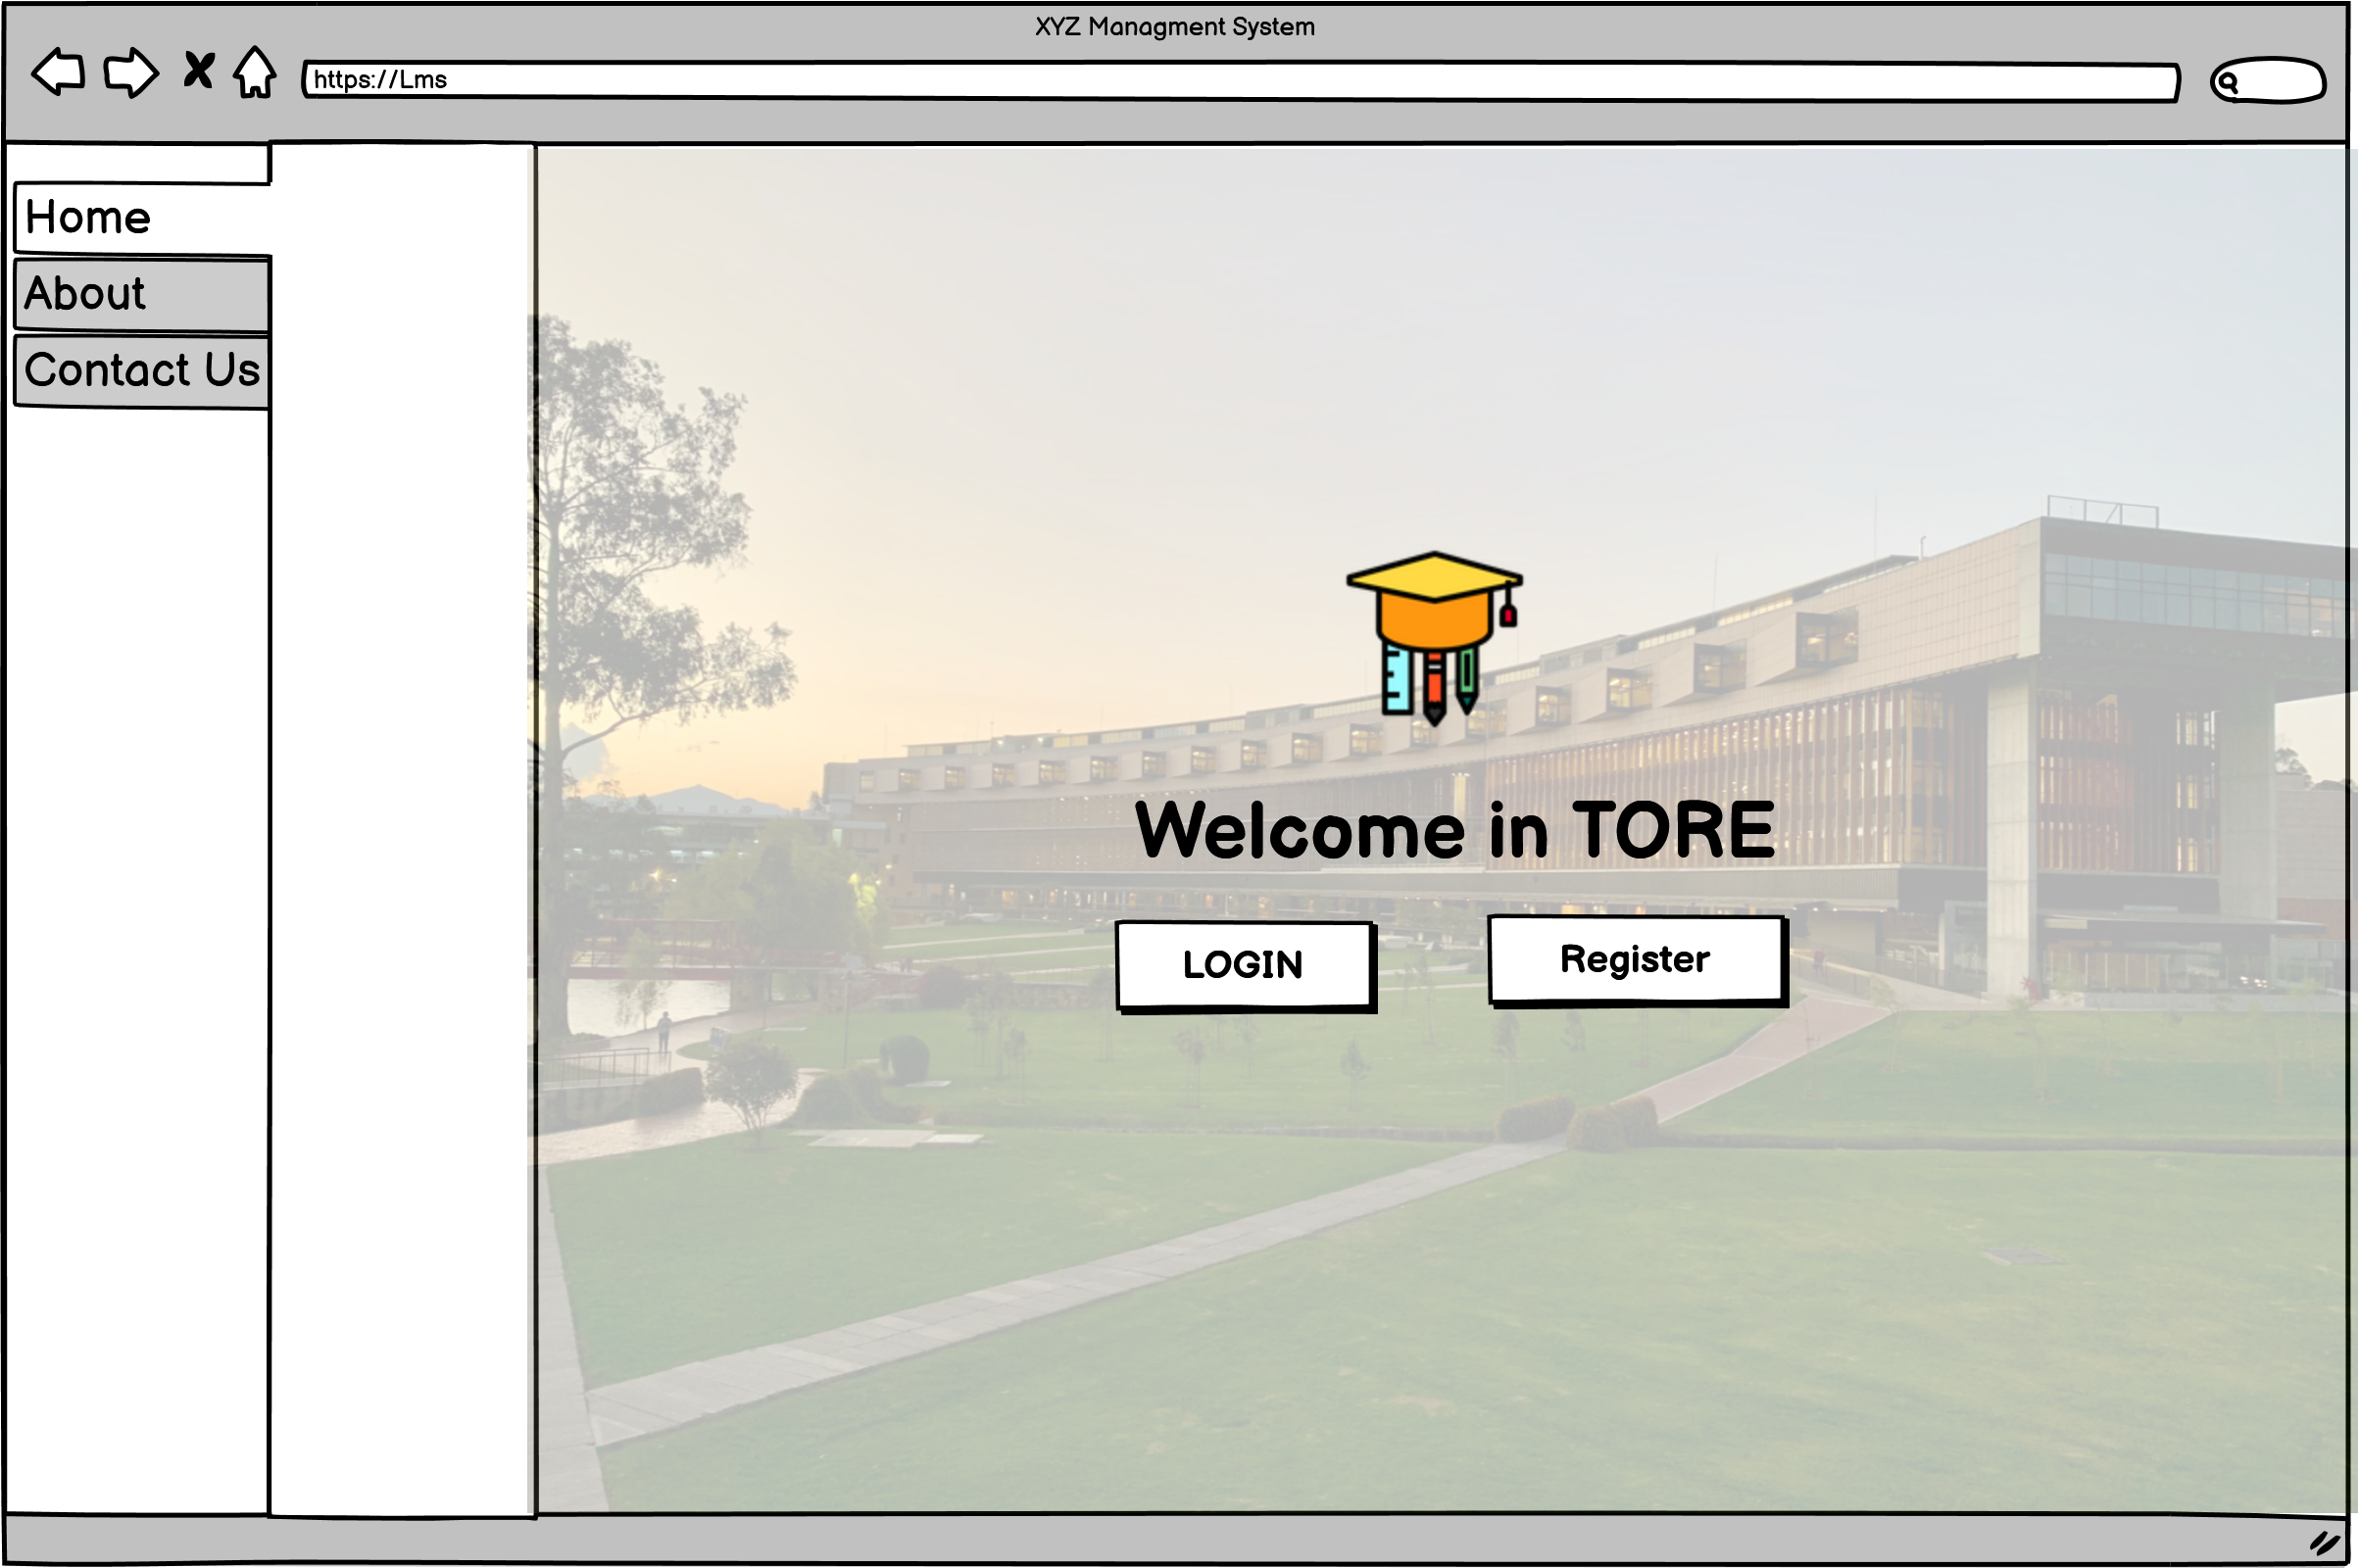
\includegraphics[width=18cm, height=11cm]{HW_1/images/New Wireframe 1.png}


\subsection{Post Material}

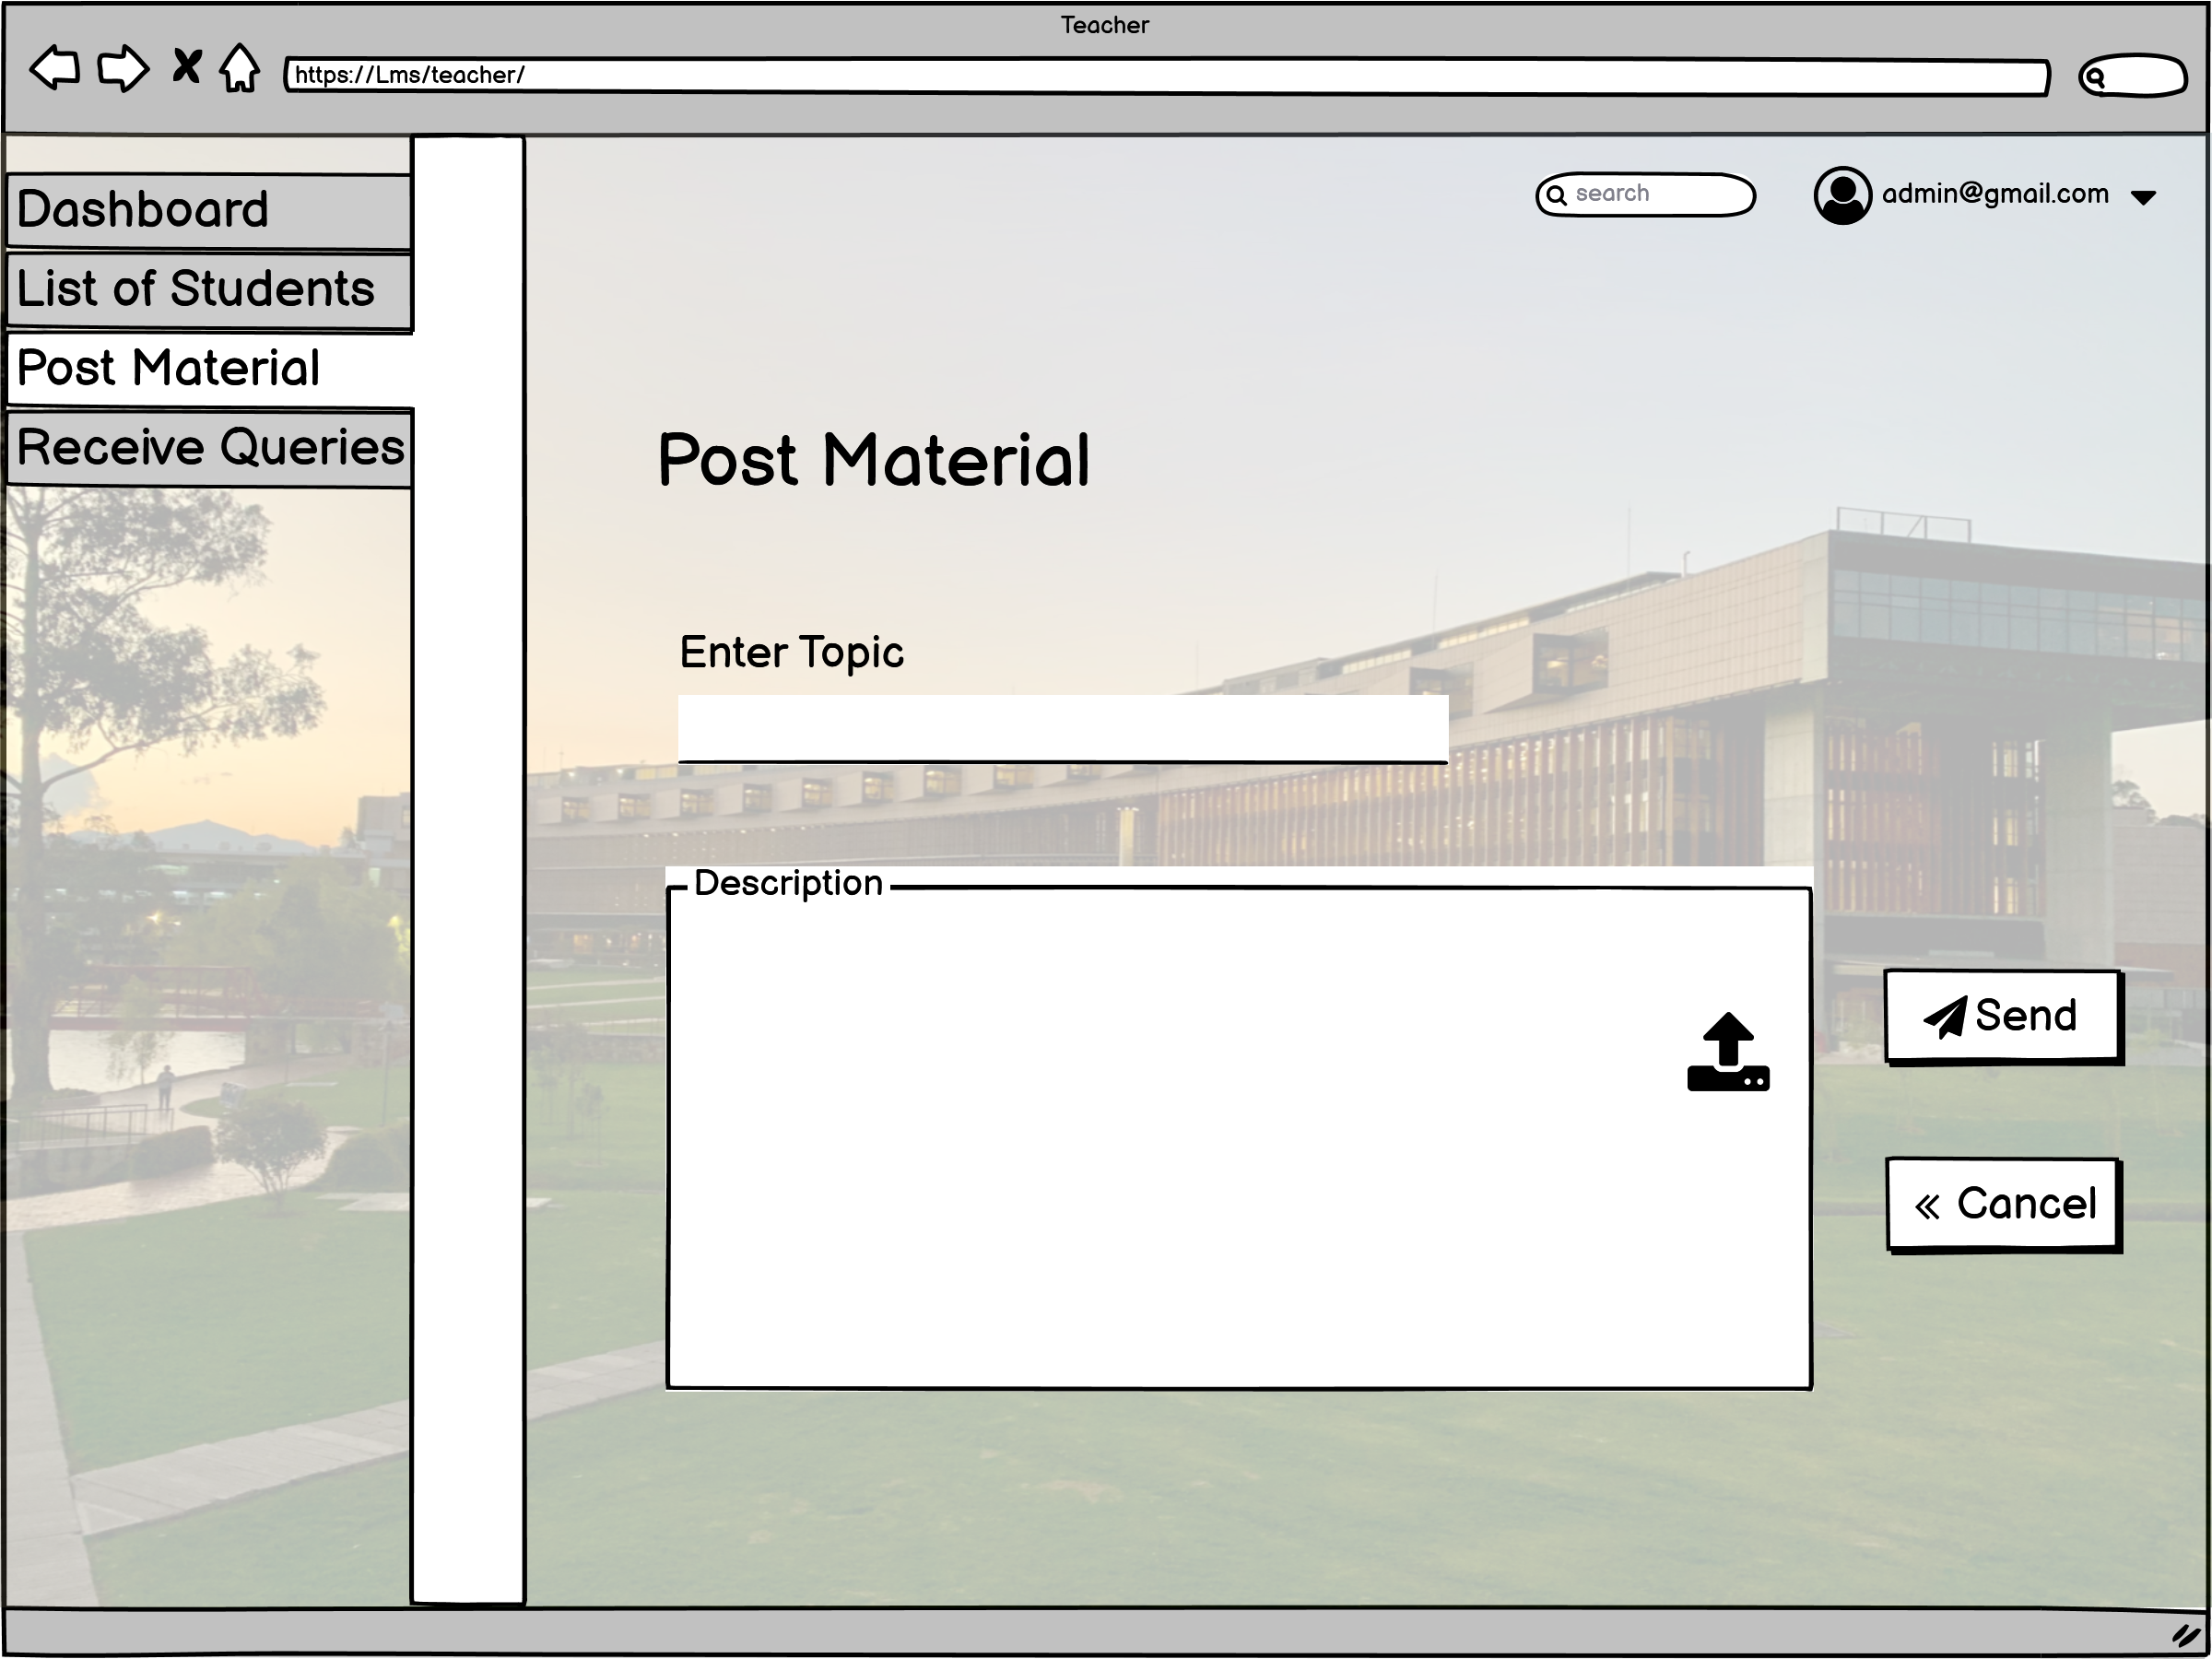
\includegraphics[width=18cm, height=11cm]{HW_1/images/Post Material.png}

\subsection{Register Wireframe}

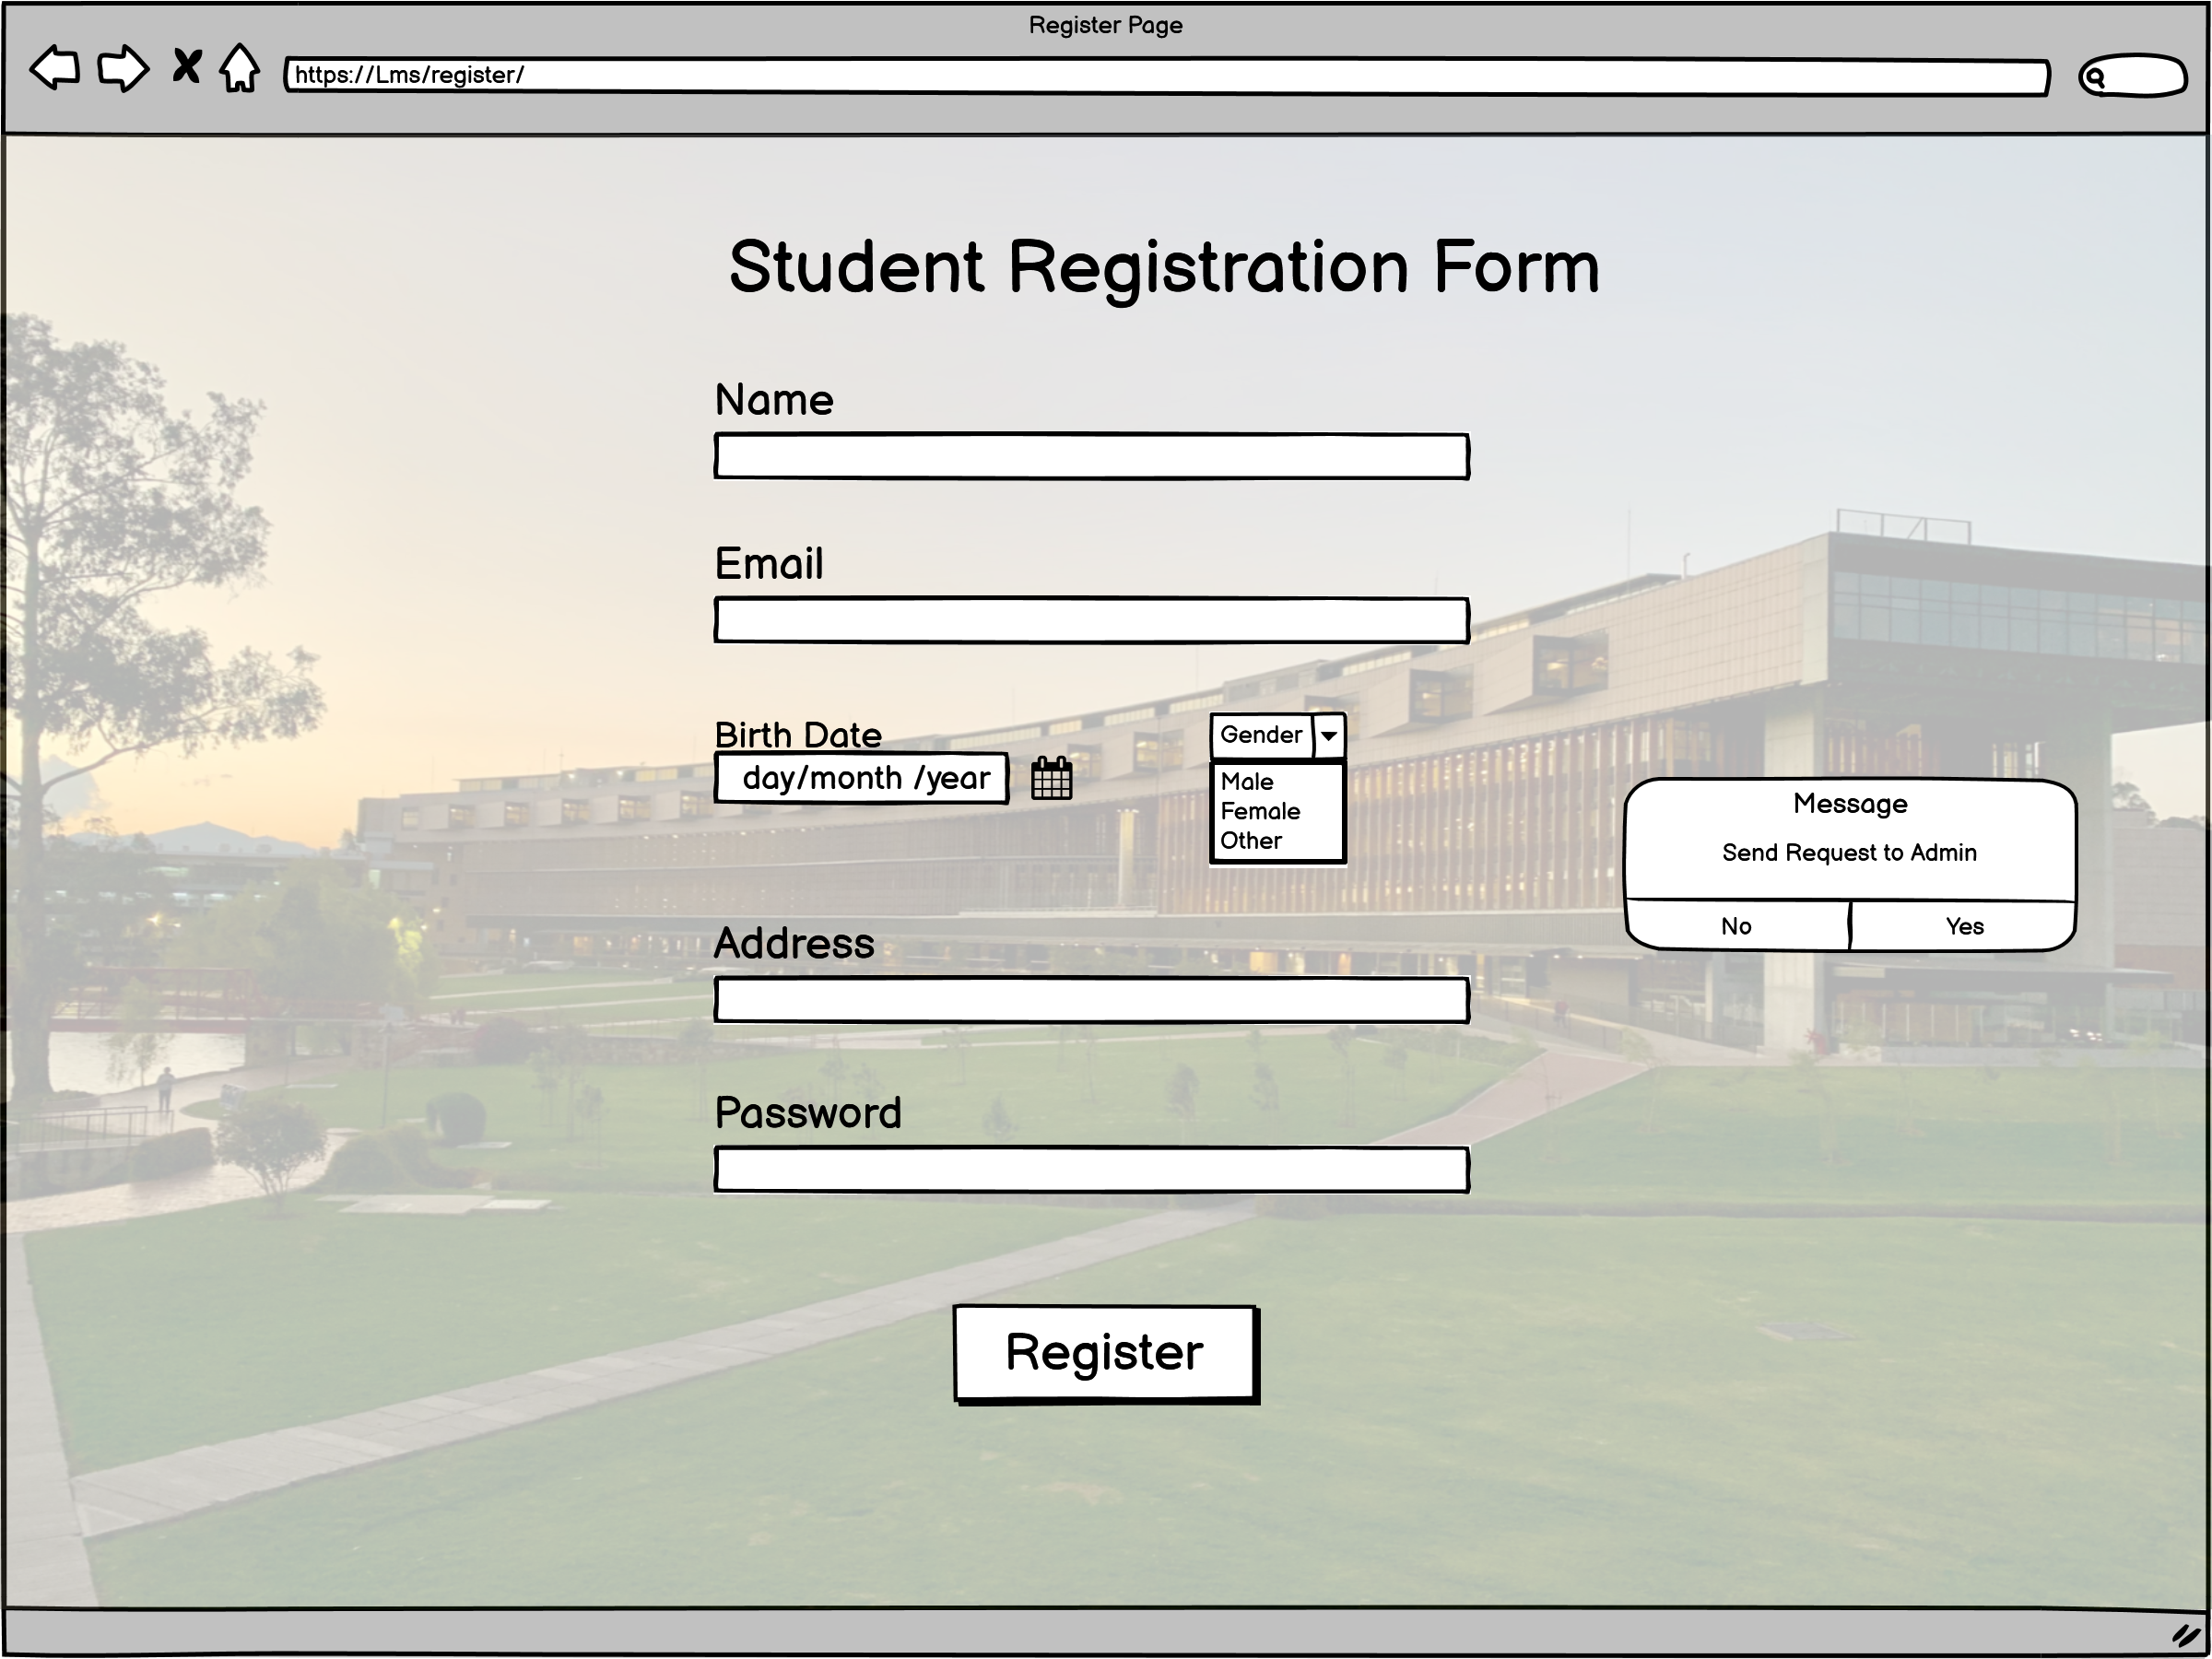
\includegraphics[width=18cm, height=11cm]{HW_1/images/Register Wireframe.png}

\subsection{Request for Course}

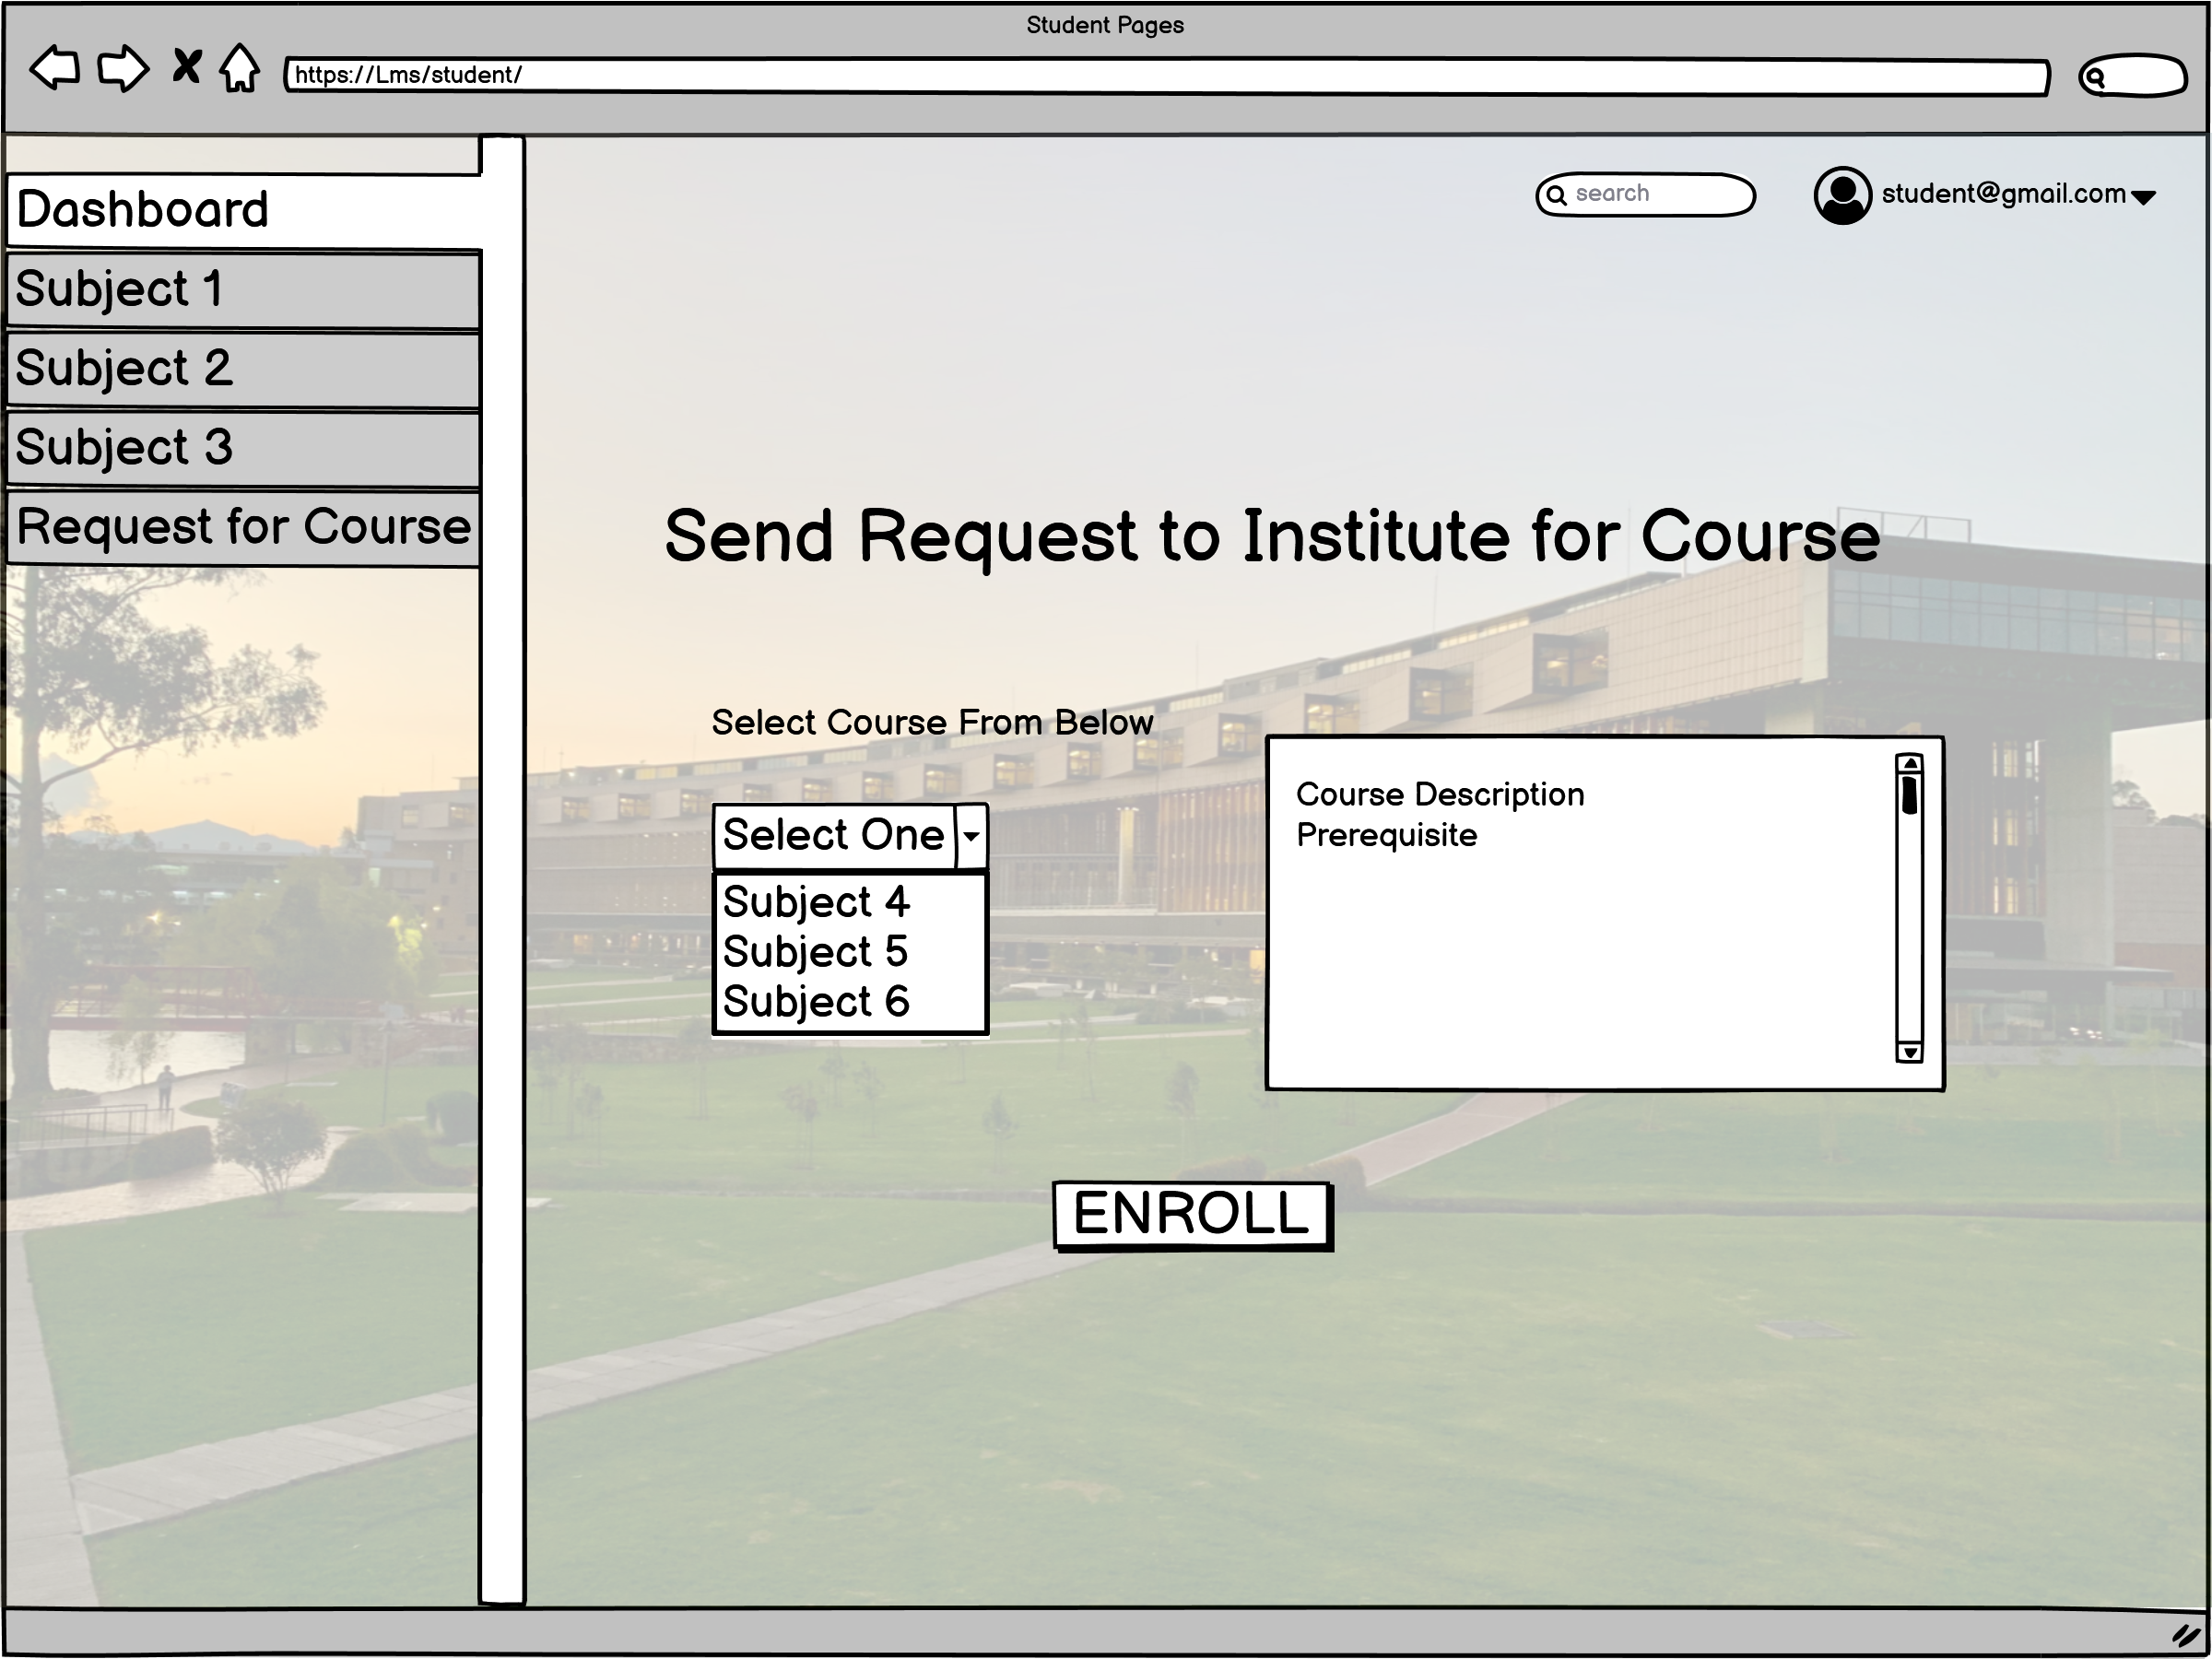
\includegraphics[width=18cm, height=11cm]{HW_1/images/Request for Course.png}

\subsection{Dashboard for Student}

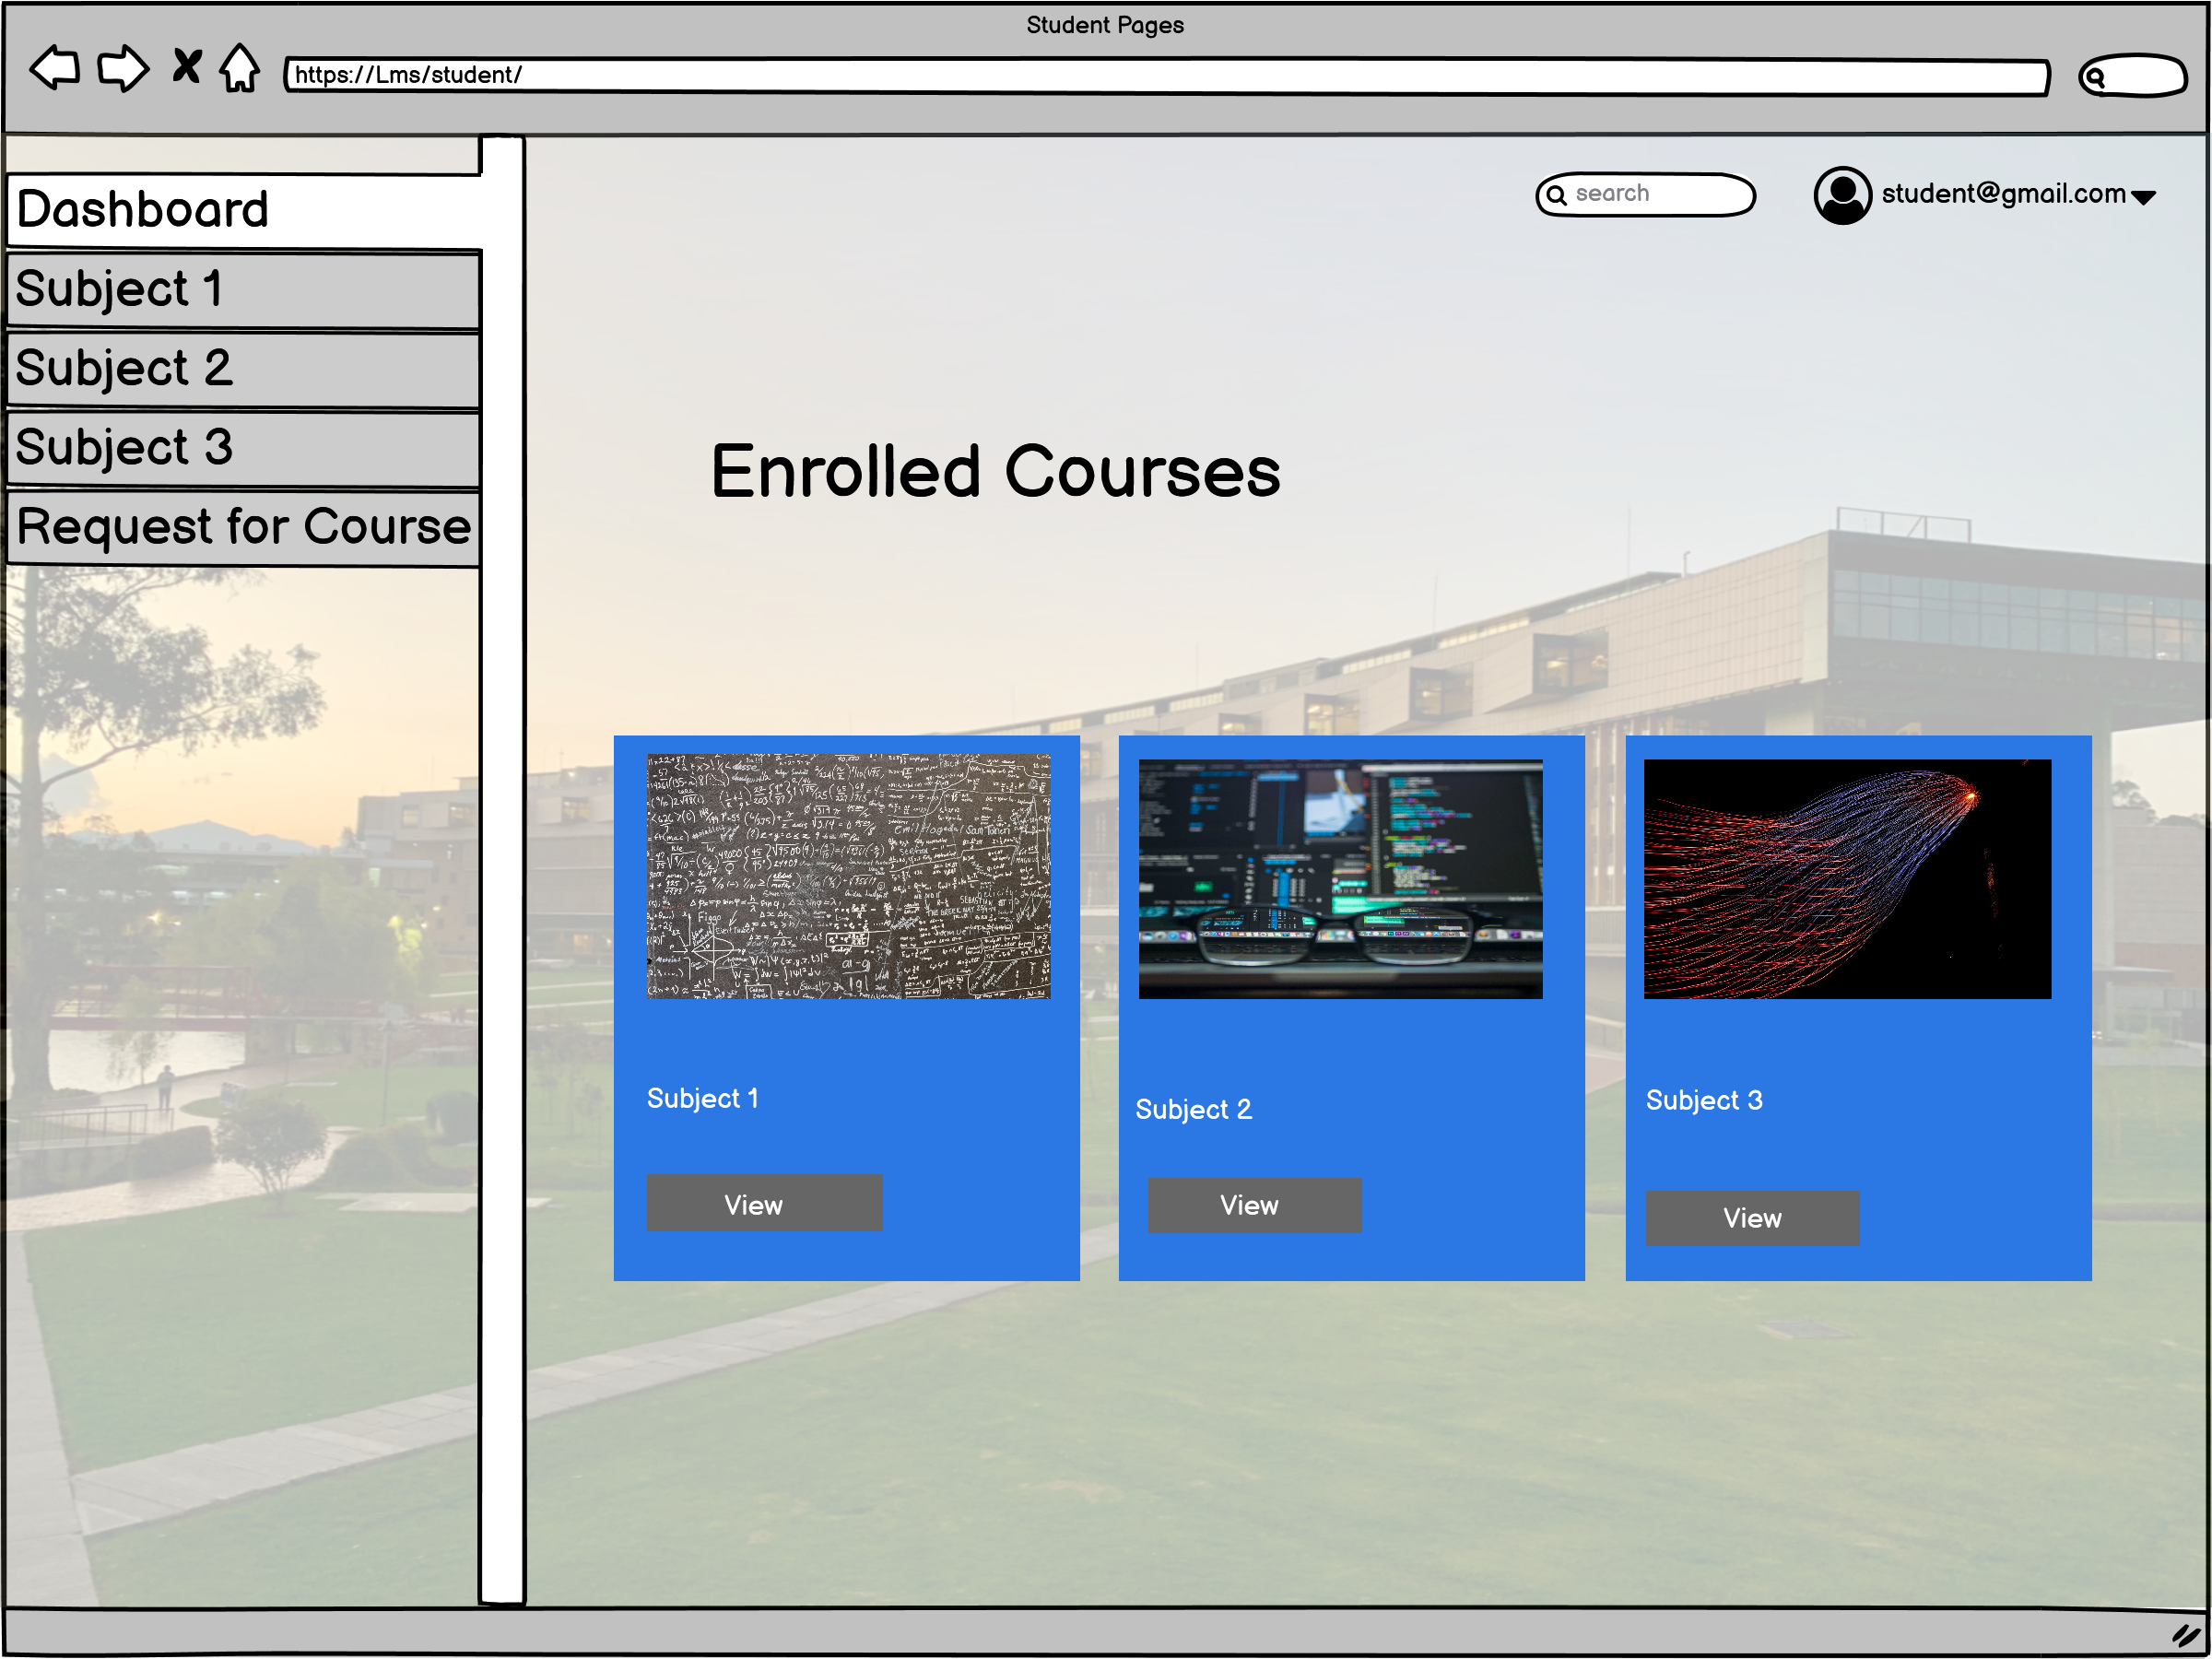
\includegraphics[width=18cm, height=11cm]{HW_1/images/Student Form.png}

\subsection{Send query to teacher}

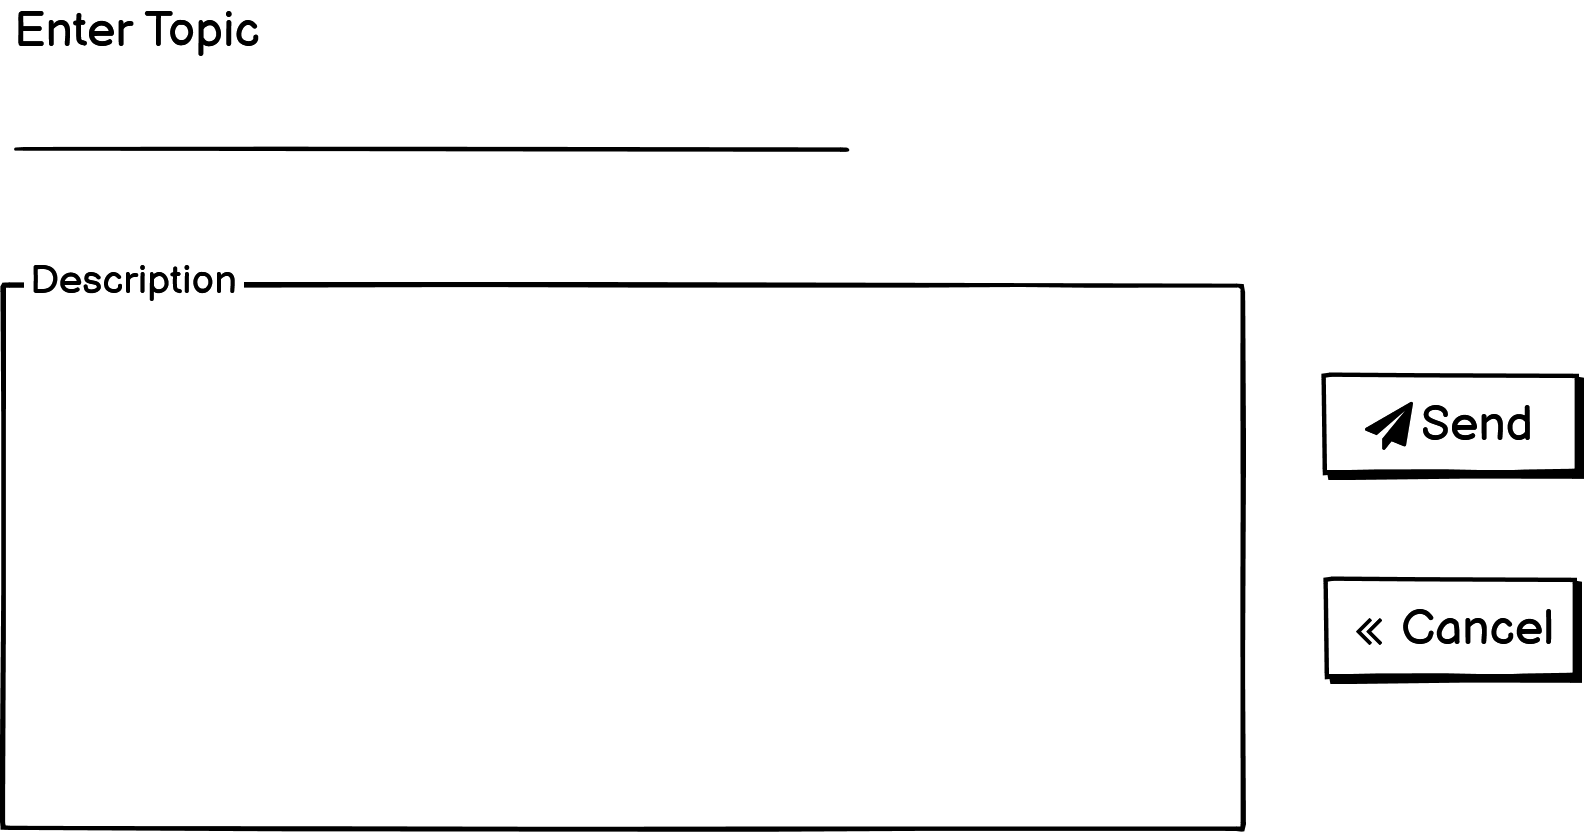
\includegraphics[width=18cm, height=11cm]{HW_1/images/Student Form_2.png}

\subsection{Subject Area}

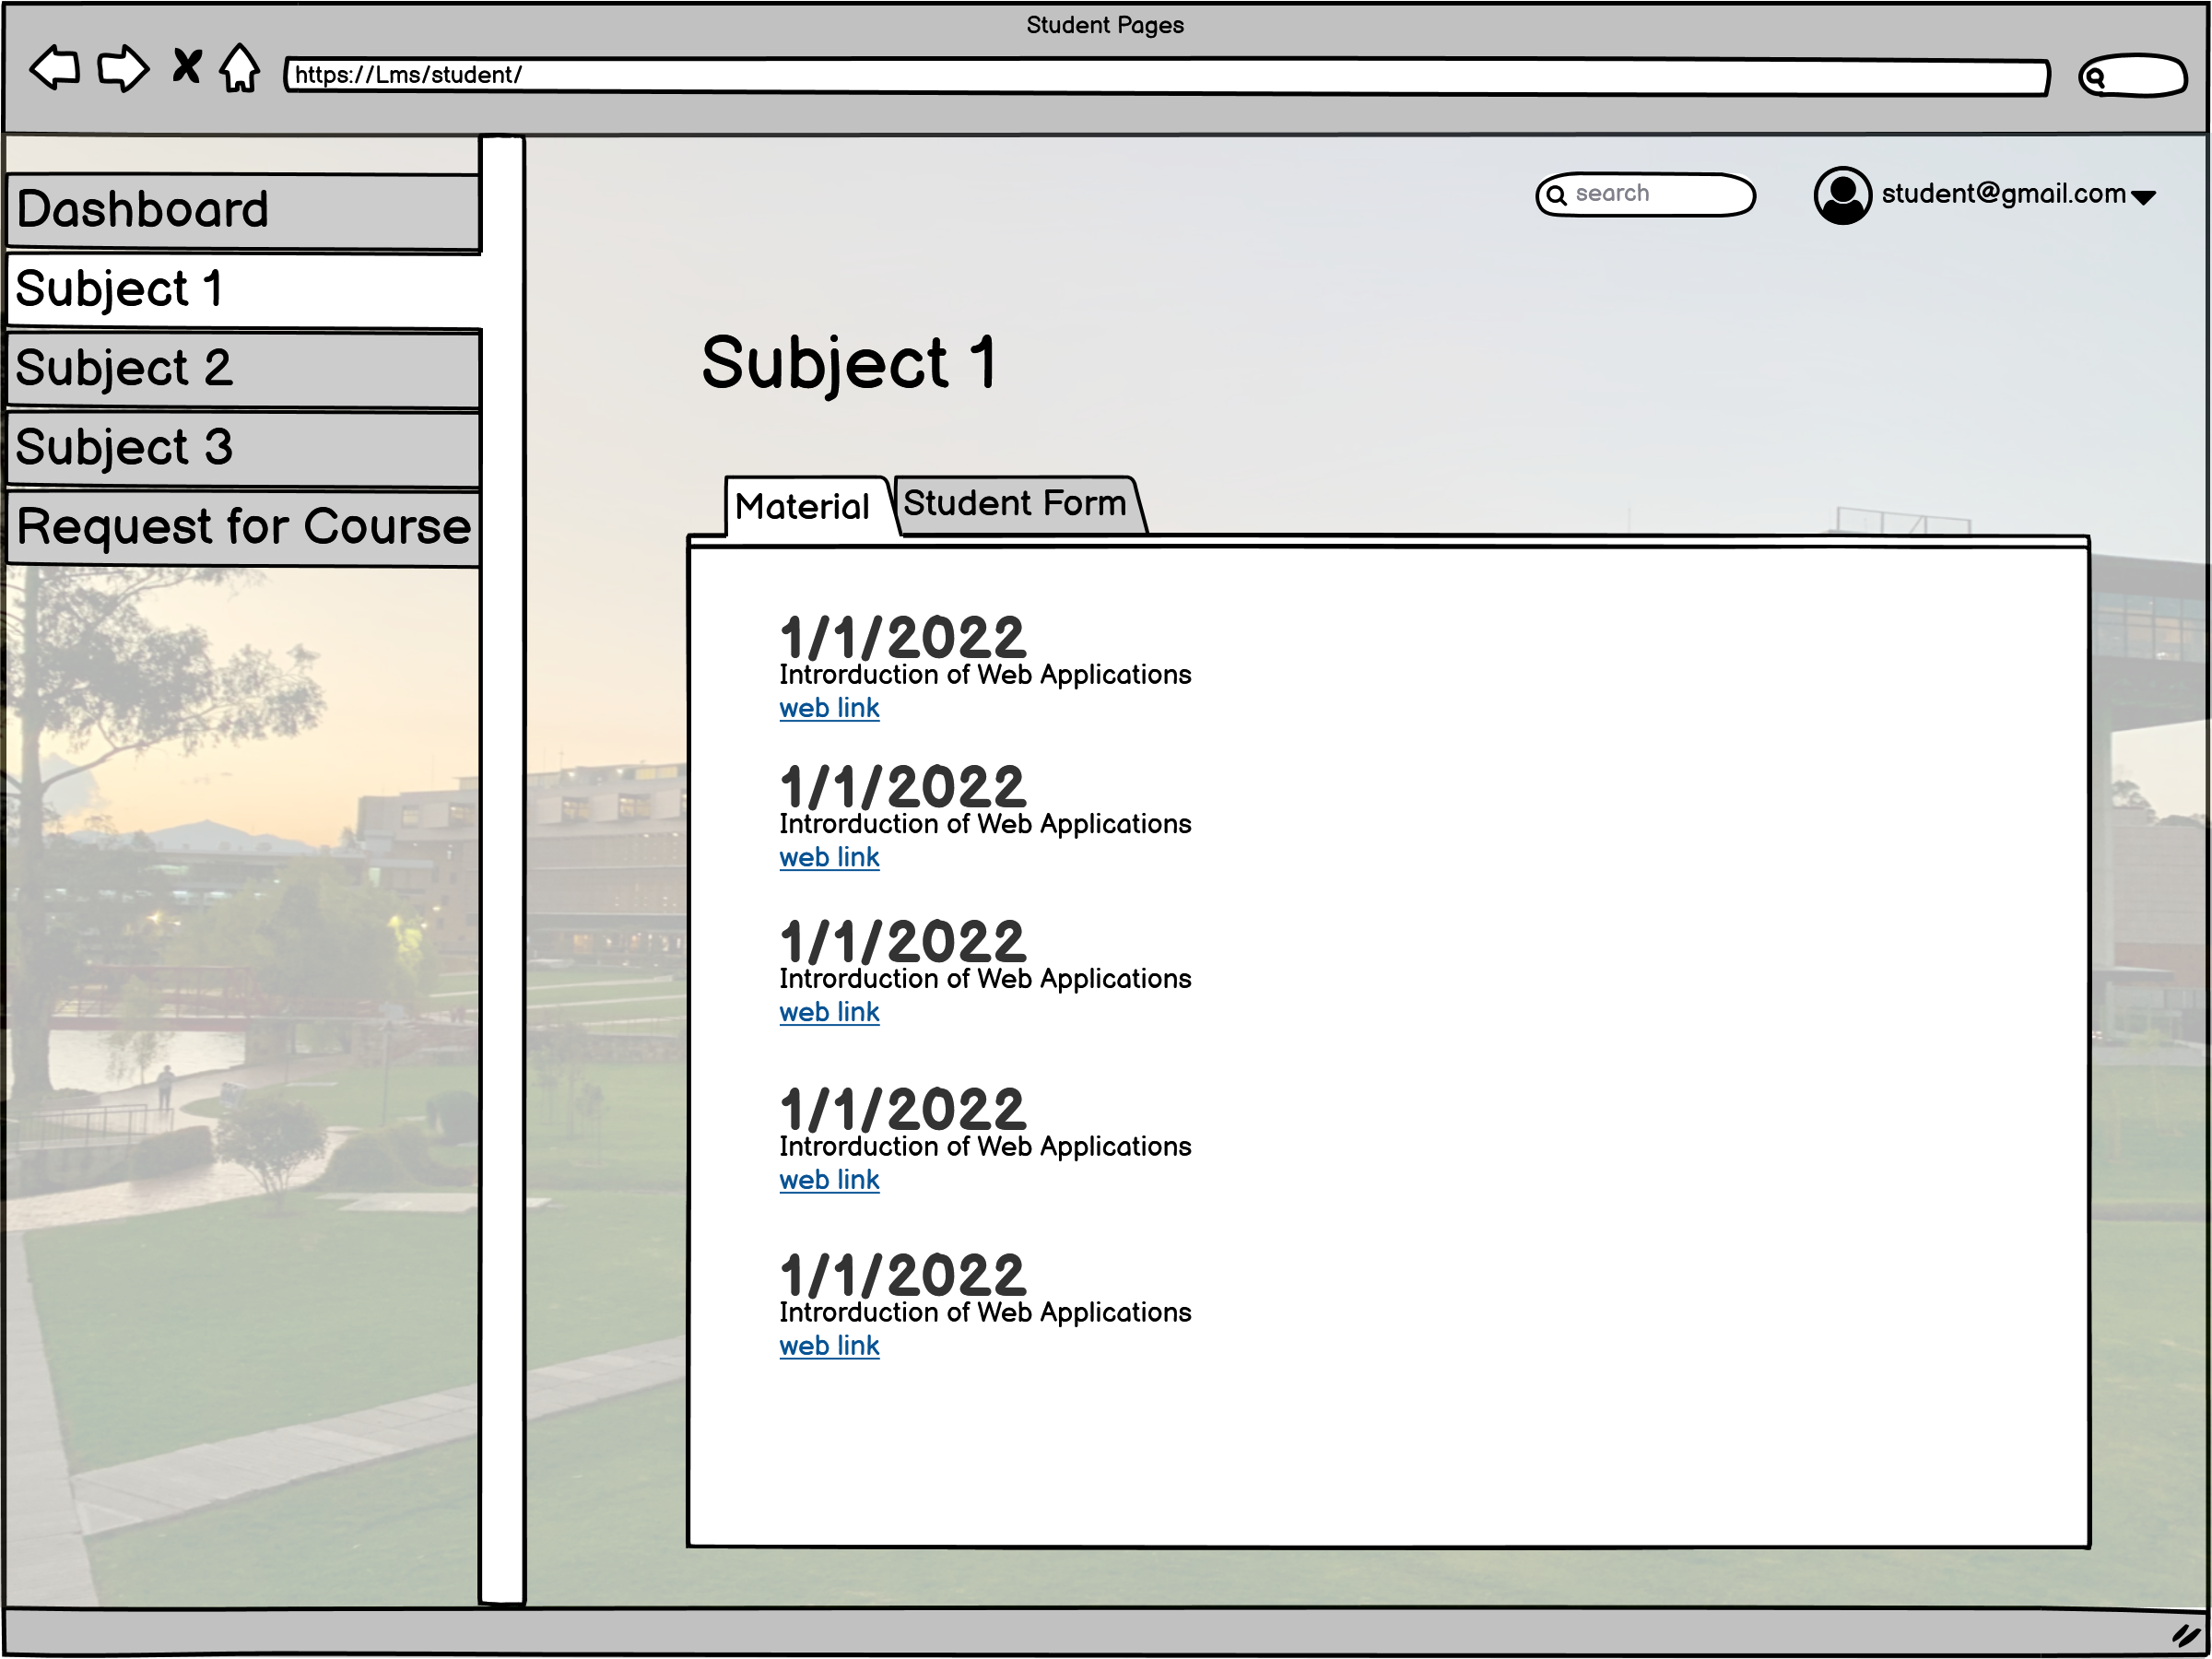
\includegraphics[width=18cm, height=11cm]{HW_1/images/Subject 1 student.png}

\subsection{Teacher Dashboard}

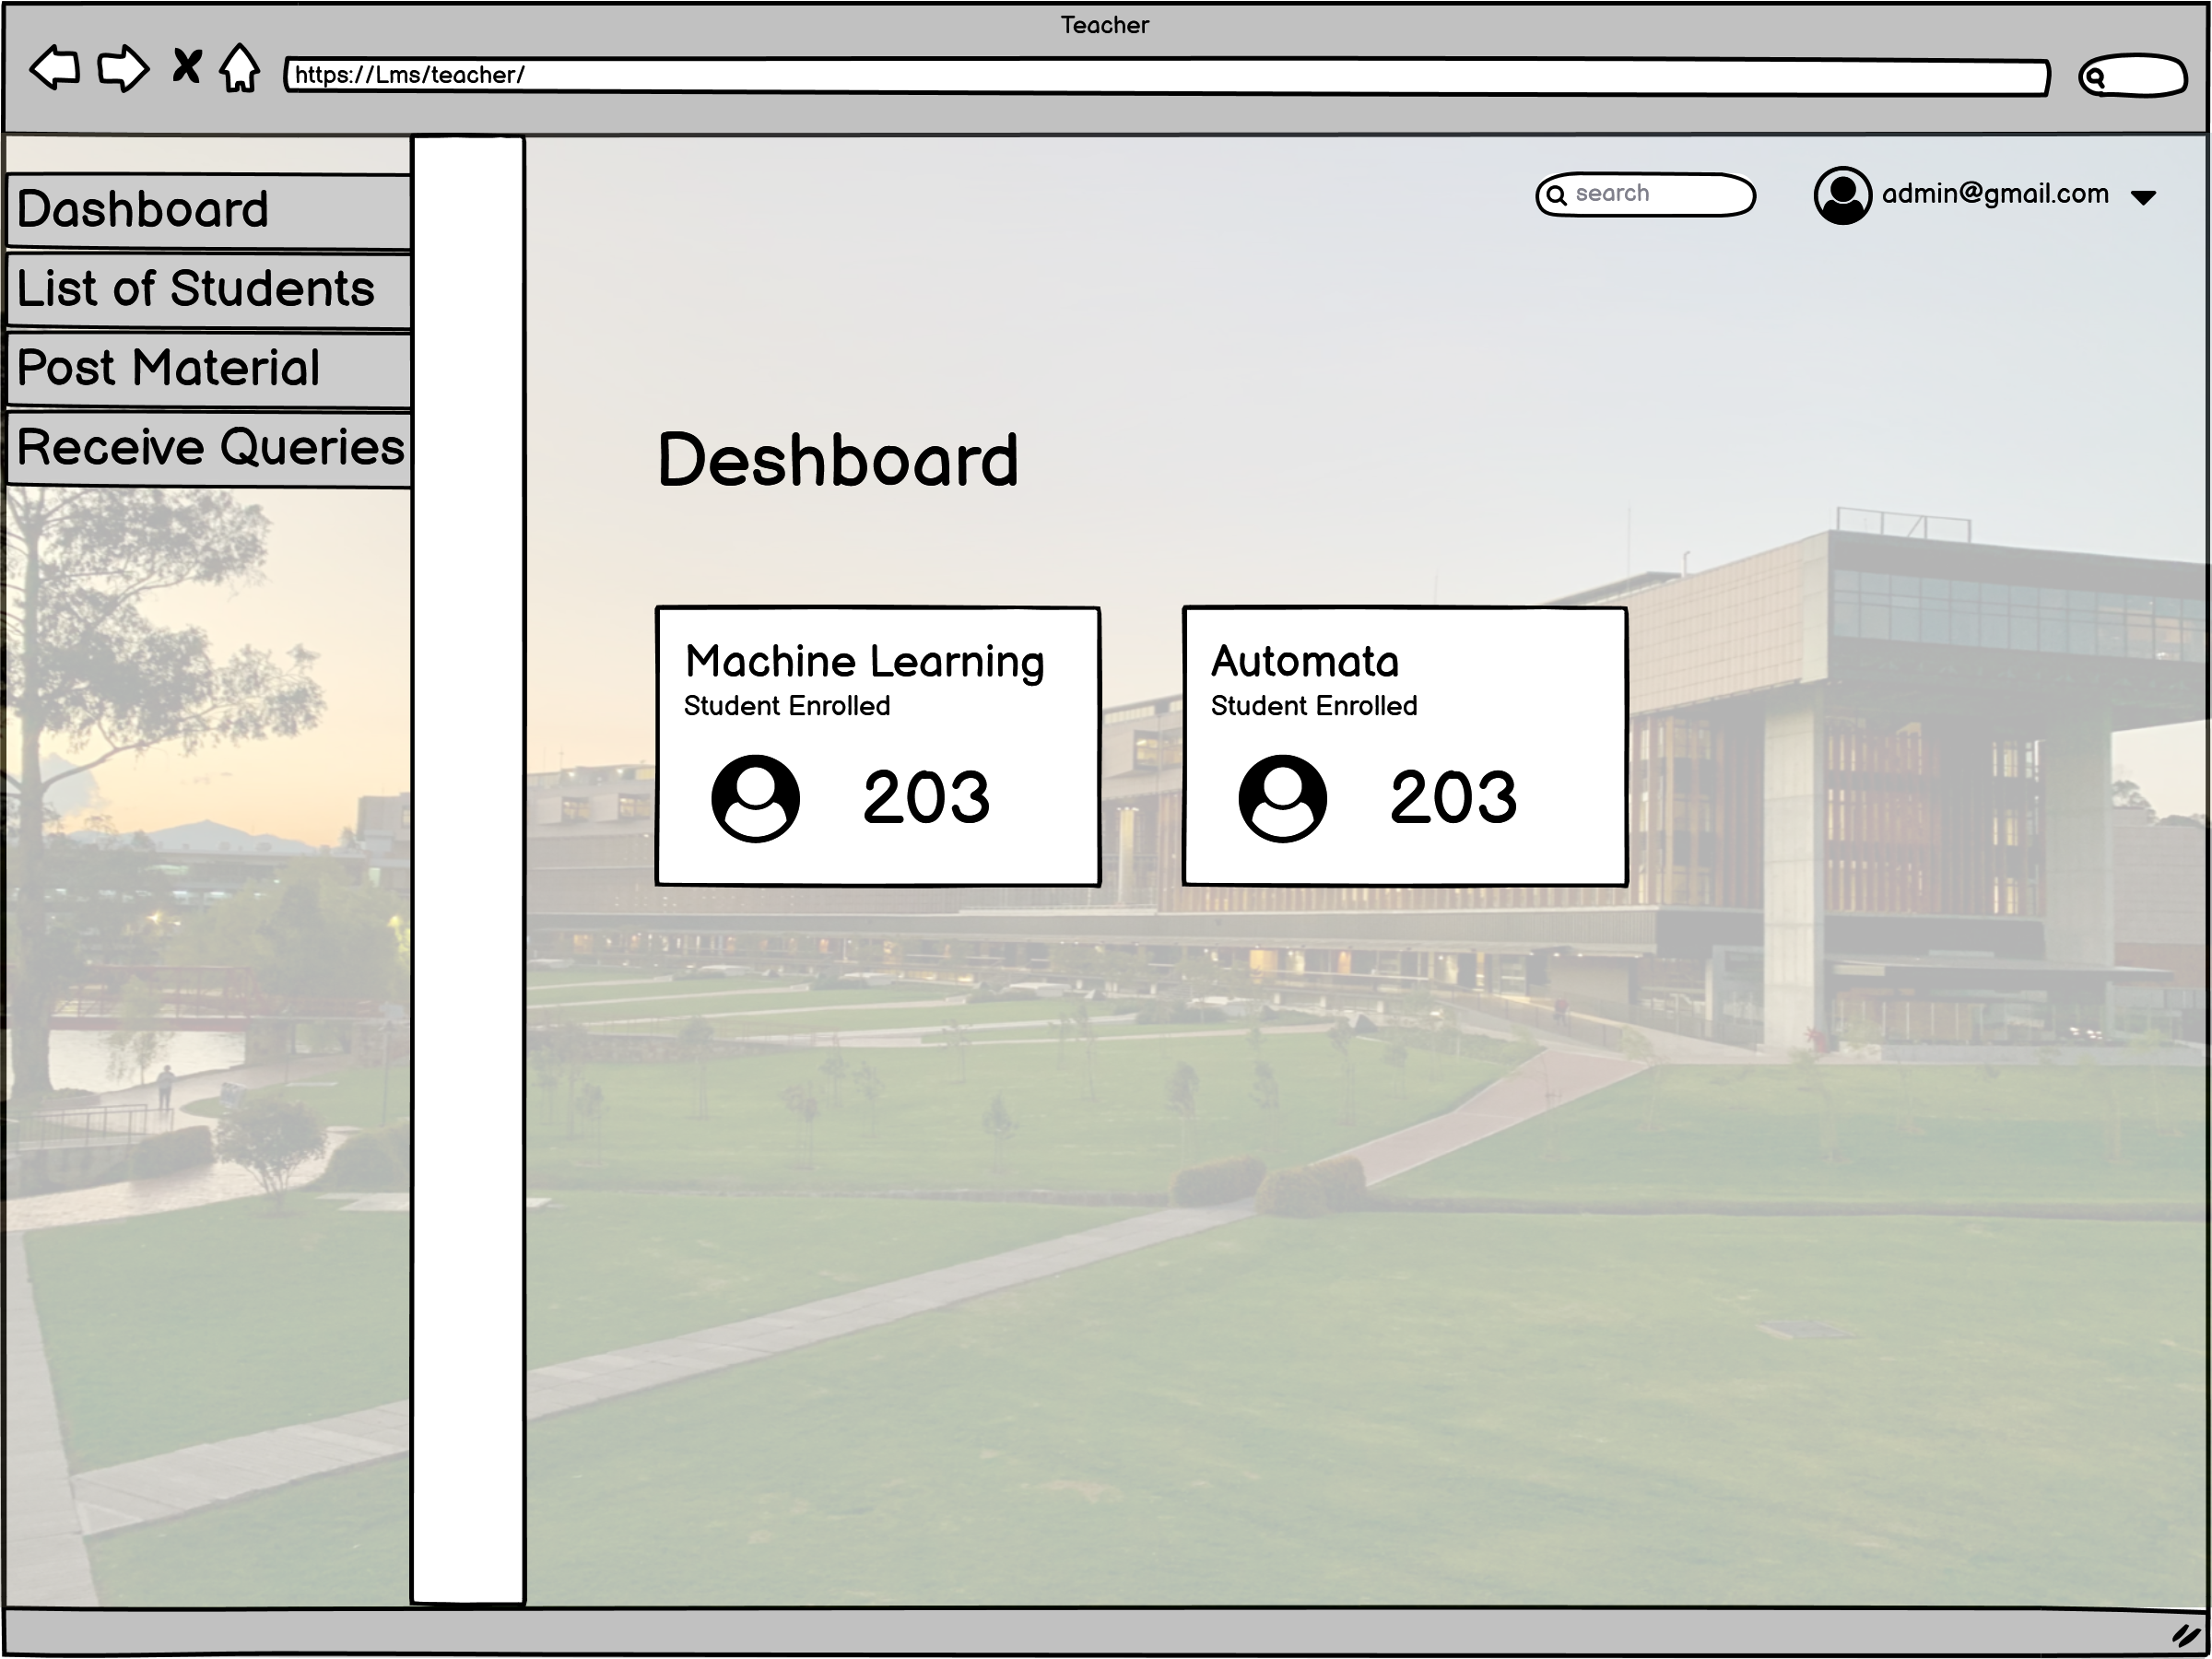
\includegraphics[width=18cm, height=11cm]{HW_1/images/Teacher Deshboard.png}

